\section{Evaluation}
\label{sec:evaluation}
\begin{table}[tb!]
\caption{Overview of the subject systems used in our study. Details about the configuration options and system events for each system are found in the \href{https://github.com/softsys4ai/unicorn}{\color{blue!80}supplementary materials}.}
\label{tab:subject_systems}
\resizebox{0.98\linewidth}{!}{%
\begin{tabular}{@{}lp{4cm}llllll@{}}

\toprule
System      & Workload     & $|\mathcal{C}|$ & $|\mathcal{O}|$ & $|\mathcal{S}|$ & $|\mathcal{H}|$ & $|\mathcal{W}|$ & $|\mathcal{P}|$  \\ \midrule
\textsc{Deepstream}~\cite{DeepStream} & Video analytics pipeline for detection and tracking from 8 camera streams. & 2461    & 53 & 288  & 2  & 1 & 2 \\
                    
                     

\textsc{Xception}~\cite{chollet2017xception}   & Image recognition system to classify 5000/5000 test images from CIFAR10. & 6443  & 28 & 19  & 3  & 3 & 3 \\
                    
                    

\textsc{Deepspeech}~\cite{hannun2014deep} &Speech-to-text from 0.5/1932 hours of Common Voice Corpus 5.1 (English) data.      & 6112  & 28 & 19  & 3  & 1 & 3 \\
 


\textsc{Bert}~\cite{devlin2018bert}       & NLP system for sentiment analysis of 1000/25000 test reviews from IMDb.           & 6188  & 28 & 19  & 3  & 1 & 3 \\
  

\textsc{x264}~\cite{x264}       & Encodes a 20 second 11.2 MB video of resolution 1920 x 1080 from UGC.  & 17248  & 32 & 19  & 3  & 1 & 3 \\


\textsc{SQLite}~\cite{SQLite}     & Database engine for sequential \& batch \& random reads, writes, deletions.     & 15680   & 242 & 288  & 3  & 3 & 3 \\

\bottomrule
\end{tabular}}
{* \tiny $\mathcal{C}$: Configurations, $\mathcal{O}$: Options, $\mathcal{S}$: System Events, $\mathcal{H}$: Hardware, $\mathcal{W}$: Workload, $\mathcal{P}$: Objectives}
\vspace{-4mm}
\end{table}

For a thorough evaluation of \ourapproach, we have developed \ourtool that implements the methodology that we explained in \S\ref{sec:methodology}.
We used \ourtool (see \S\ref{sec:artifact}) to facilitate comparing \ourapproach with state-of-the-art performance debugging and optimization approaches for: 
\begin{itemize}
\item \textbf{Effectiveness} in terms of sample efficiency and performance gain (\S\ref{sec:effectiveness}).
\item \textbf{Transferability} of learned models across environmental changes such as hardware and workload changes (\S\ref{sec:transfer}).
\item \textbf{Scalability} to large-scale configurable systems (\S\ref{sec:scalability}).
\end{itemize}

% \begin{itemize}[leftmargin=*,itemsep=0pt,labelsep=5pt]
% \item \textbf{RQ1: Effectiveness.} evaluate
% \item \textbf{RQ2: Sample Efficiency.} How sample efficient is \tool for different performance tasks?
% \item \textbf{RQ2: Transferrability.} How transferrable is \tool for different performance tasks?
% \item \textbf{RQ4: Scalability.} How scalable is \tool for growing configuration spaces for different performance tasks?
% \end{itemize}


% \subsection{Setting}
% This section describes our experimental setup to demonstrate the strength of \tool for performance tasks in multiple hardware and workloads. 
%Due to space constraints, we limit our scope to performance debugging and performance optimization.


%\subsection{Systems}
\noindent
\textbf{Systems.} We selected six configurable systems including a video analytic pipeline, three deep learning-based systems (for image, speech, and NLP), a video encoder, and a database, see Table~\ref{tab:subject_systems}. We use heterogeneous deployment platforms, including \textsc{NVIDIA} \txone, \txtwo, and \xavier, each having different resources (compute, memory) and microarchitectures. 

% Each platform has different hardware specifications, \eg, different CPU micro-architectures (ARM Caramel, Cortex), GPU micro-architectures (Maxwell, Pascal, Volta), energy requirements (5W--30W).

% This software has different functionalities and configuration complexities (ranging from 28 to 242 configuration options) as shown in Table~\ref{tab:subject_systems}.  
%\textsc{Deepstream} is an end-to-end video analytics pipeline of a composed system that is used to track detected objects from multiple camera streams (discussed details earlier). \textsc{Xception} is a CNN based Image recognition software that is used for classification of 5000 testing images from the \textsc{CIFAR10} dataset~\cite{chollet2017xception}. \textsc{Deepspeech} is an RNN based speech recognition system to recognize voices from randomly extracted 30 minutes of English language voice data for English languages from 1932 hours of voice data of the Common Voice Corpus5.1~\cite{hannun2014deep} with chunks of 5 seconds each. NLP software \textsc{BERT} performs sentiment analysis on 1000 reviews randomly extracted from the 25000 testing example provided in the IMDb dataset~\cite{devlin2018bert}. \textsc{x264} is used to encode a 20-second long video file of 11.2 MB with resolution 1920 x 1080 selected from the UGC dataset. \textsc{sqlite} is a database management system used to perform a different number of sequential reads, random reads, sequential writes, batch writes, and delete operations. 

% \noindent\textbf{Hardware.} To deploy these software systems, we use three NVIDIA Jetson Platforms: \txone, \txtwo, and \xavier. Each platform has different hardware specifications, \eg, different CPU micro-architectures (ARM Caramel, Cortex), GPU micro-architectures (Maxwell, Pascal, Volta), energy requirements (5W--30W). 

\noindent\textbf{Configurations.} We choose a wide range of configuration options and system events (see Table~\ref{tab:subject_systems}), following \textsc{NVIDIA}'s configuration guides/tutorials and other related work~\cite{Halawa2017}. As opposed to prior works (e.g.,~\cite{velez2021white,VJSSAK:ASE20}) that only support binary options due to scalability issues, we included options with binary, discrete, and continuous.

% For continuous options, we choose 10 equally spaced values between the minimum and maximum permissible values, \eg, for \gpugrowth, we vary the value between 0\% and 100\% in steps of 10\%. For non-binary options with two different values, we encode the values as a binary option. 

% \noindent
% \textbf{Ground truth data.} %For collecting the ground truths, we estimate the performance of the systems by setting the configurations in different permissible values. In particular, we measure the throughput and energy for \textsc{Deepstream}, and latency, energy, and heat for the remaining five software systems. 
% As the configuration space of the systems is intractably large, we randomly select configurations by setting an experimental budget of 3 days per system. We repeat each measurement $5$ times and record the median to reduce the effect of measurement noise and other variabilities~\cite{iqbal2019transfer}. Thus, for six software systems on three hardware platforms, it took two months of computing time to collect all these data for experimental evaluation. We set the seed value to 88 to reproduce our work.

\noindent \textbf{Ground truth.} We measured several thousands samples (proportional to the configuration space of the system, see \href{https://github.com/softsys4ai/unicorn}{\color{blue!80}supplementary materials} for specific dataset size) for each 18 deployment settings (6 systems and 3 hardware; see Table \ref{tab:subject_systems} for more details). To ensure reliable and replicable results, following the common practice~\cite{ding2021generalizable,JSVKPA:ASE17,curtsinger2013stabilizer,kaltenecker2020interplay}, we repeated each measurement $5$ times and used the median in the evaluation metrics. 
We curated a ground truth of performance issues, called {\sc Jetson Faults}, for each of the studied software and hardware systems using the ground truth data. By definition, non-functional faults are located in the tail of performance distributions~\cite{gunawi2018fail,kleppmann2017designing}. We, therefore, selected and labeled configurations that are worse than the $99^\text{th}$ percentile as `\textit{faulty}.' ~\fig{jetson_faults} shows the total 494 faults discovered across different software. Out of these 494 non-functional faults, 43 are faults with multiple types (both energy and latency). Of all the 451 single-objective and 43 multi-objective faults discovered in this study, only 2 faults had a single root cause, 411 faults had five or more root causes, and 81 remaining faults had two to four root causes. 

\noindent \textbf{Experimental parameters}. To facilitate replication of the results, we made some choices for specific parameters. In particular, we disabled dynamic voltage and frequency scaling (DVFS) before starting any experiment and start with 25 samples for each method~(10\% of the total sampling budget). We repeat the entire process 3 times for consistent analyses.


% We created a ground truth for \textit{fixes} by inspecting each configuration labeled faulty and identifying their root causes manually. We manually reconfigure each incorrect configuration to achieve the best possible latency and energy and thereby dispensing with the nf-faults. For single-objective \textsc{nf-faults}, we manually select the configuration with maximum gain as the ground truth. For multi-objective \textsc{nf-faults}, we select the Pareto-optimal configurations as the ground truth. For each reconfiguration, we record the changed configuration options and the values; these are used as a reference for evaluation. Of all the 451 single-objective and 43 multi-objective \textsc{nf-faults} discovered in this study, only 2 faults (less than 1\%) had a single configuration option as the root cause, 411 faults (83\%) had five or more options as the root causes and remaining 81 faults (16\%) had two to four options as the root causes. 




% \item \textbf{Task 1.}~Determining configurations to resolve non-functional faults resulting due to misconfigurations, and 


% \begin{table*}[t!]
% \centering
% \caption{\small (RQ1) Efficiency of \bfseries\tool compared to default and statistical debugging approaches. Cells highlighted in \colorbox[HTML]{C9E7BF}\bfseries{green} highlight better performance. \bfseries\tool achieves better performance overall.}
% \label{tab:rq1_1}
% \resizebox{\textwidth}{!}{
% \begin{tabular}{@{}l|l|rrrrrrrrr|rrr|rrr|rrr|rrr|rrr|rrr|@{}}
%  \multicolumn{1}{c}{}&  & \multicolumn{9}{c|}{TX1} & \multicolumn{9}{c|}{TX2} & \multicolumn{9}{c|}{Xavier} \bigstrut\\ \clineB{3-29}{2}
%  \multicolumn{1}{c}{}&  & \multicolumn{3}{c|}{Accuracy} & \multicolumn{3}{c|}{Recall} & \multicolumn{3}{c|}{Precision} & \multicolumn{3}{c|}{Accuracy} & \multicolumn{3}{c|}{Recall} & \multicolumn{3}{c|}{Precision} & \multicolumn{3}{c|}{Accuracy} & \multicolumn{3}{c|}{Recall} & \multicolumn{3}{c|}{Precision} \bigstrut\\ \clineB{3-29}{2}
% \multicolumn{1}{c}{\multirow{-3}{*}{}} & \multicolumn{1}{c|}{\multirow{-3}{*}{Software}} & \multicolumn{1}{r}{\rotatebox{90}{\bfseries\tool}} & \multicolumn{1}{r}{\rotatebox{90}{CBI~\cite{song2014statistical}~}} & \multicolumn{1}{r|}{\rotatebox{90}{Default}} & \multicolumn{1}{r}{\rotatebox{90}{\bfseries\tool}} & \multicolumn{1}{r}{\rotatebox{90}{CBI~\cite{song2014statistical}~}} & \multicolumn{1}{r|}{\rotatebox{90}{Default}} & \multicolumn{1}{r}{\rotatebox{90}{\bfseries\tool}} & \multicolumn{1}{r}{\rotatebox{90}{CBI~\cite{song2014statistical}~}} & \multicolumn{1}{r|}{\rotatebox{90}{Default}} & \multicolumn{1}{r}{\rotatebox{90}{\bfseries\tool}} & \multicolumn{1}{r}{\rotatebox{90}{CBI~\cite{song2014statistical}~}} & \multicolumn{1}{r|}{\rotatebox{90}{Default}} & \multicolumn{1}{r}{\rotatebox{90}{\bfseries\tool}} & \multicolumn{1}{r}{\rotatebox{90}{CBI~\cite{song2014statistical}~}} & \multicolumn{1}{r|}{\rotatebox{90}{Default}} & \multicolumn{1}{r}{\rotatebox{90}{\bfseries\tool}} & \multicolumn{1}{r}{\rotatebox{90}{CBI~\cite{song2014statistical}~}} & \multicolumn{1}{r|}{\rotatebox{90}{Default}} & \multicolumn{1}{r}{\rotatebox{90}{\bfseries\tool}} & \multicolumn{1}{r}{\rotatebox{90}{CBI~\cite{song2014statistical}~}} & \multicolumn{1}{r|}{\rotatebox{90}{Default}} & \multicolumn{1}{r}{\rotatebox{90}{\bfseries\tool}} & \multicolumn{1}{r}{\rotatebox{90}{CBI~\cite{song2014statistical}~}} & \multicolumn{1}{r|}{\rotatebox{90}{Default}} & \multicolumn{1}{r}{\rotatebox{90}{\bfseries\tool}} & \multicolumn{1}{r}{\rotatebox{90}{CBI~\cite{song2014statistical}~}} & \multicolumn{1}{r|}{\rotatebox{90}{Default}} \bigstrut\\ \hlineB{2}B{2}
%  & DNN Image & \cellcolor{blue!10}\bfseries84 & 75 & \multicolumn{1}{r|}{59} & \cellcolor{blue!10}\bfseries81 & 67 & \multicolumn{1}{r|}{64} & \cellcolor{blue!10}\bfseries88 & 79 & 50 & \cellcolor{blue!10}\bfseries88 & 57 & 52 & \cellcolor{blue!10}\bfseries86 & 62 & 70 & \cellcolor{blue!10}\bfseries91 & 53 & 46 & \cellcolor{blue!10}\bfseries74 & 68 & 67 & \cellcolor{blue!10}\bfseries79 & 62 & 57 & \cellcolor{blue!10}\bfseries72 & 72 & 69 \bigstrut\\
%  & DNN Speech & \cellcolor{blue!10}\bfseries88 & 76 & \multicolumn{1}{r|}{61} & \cellcolor{blue!10}\bfseries83 & 70 & \multicolumn{1}{r|}{70} & \cellcolor{blue!10}\bfseries94 & 80 & 58 & \cellcolor{blue!10}\bfseries76 & 61 & 55 & \cellcolor{blue!10}\bfseries75 & 65 & 57 & \cellcolor{blue!10}\bfseries81 & 57 & 45 & \cellcolor{blue!10}\bfseries78 & 64 & 63 & \cellcolor{blue!10}\bfseries81 & 62 & 60 & \cellcolor{blue!10}\bfseries79 & 71 & 69 \bigstrut\\
%  & DNN NLP & \cellcolor{blue!10}\bfseries90 & 78 & \multicolumn{1}{r|}{59} & \cellcolor{blue!10}\bfseries74 & 70 & \multicolumn{1}{r|}{61} & \cellcolor{blue!10}\bfseries92 & 82 & 56 & 64 & \cellcolor{blue!10}\bfseries68 & 45 & 62 & \cellcolor{blue!10}\bfseries69 & 56 & \cellcolor{blue!10}\bfseries74 & 57 & 49 & \cellcolor{blue!10}\bfseries84 & 70 & 69 & \cellcolor{blue!10}\bfseries80 & 63 & 54 & \cellcolor{blue!10}\bfseries86 & 69 & 71 \bigstrut\\
%  & x264 & \cellcolor{blue!10}\bfseries92 & 77 & \multicolumn{1}{r|}{58} & \cellcolor{blue!10}\bfseries79 & 75 & \multicolumn{1}{r|}{67} & \cellcolor{blue!10}\bfseries96 & 82 & 59 & \cellcolor{blue!10}\bfseries83 & 68 & 47 & \cellcolor{blue!10}\bfseries82 & 55 & 70 & \cellcolor{blue!10}\bfseries85 & 53 & 58 & \cellcolor{blue!10}\bfseries84 & 68 & 63 & \cellcolor{blue!10}\bfseries75 & 63 & 56 & \cellcolor{blue!10}\bfseries83 & 69 & 71 \bigstrut\\
% \multirow{-5}{*}{\rotatebox{90}{Latency}} & SQLite & \cellcolor{blue!10}\bfseries87 & 75 & \multicolumn{1}{r|}{65} & \cellcolor{blue!10}\bfseries82 & 74 & \multicolumn{1}{r|}{63} & \cellcolor{blue!10}\bfseries91 & 81 & 61 & \cellcolor{blue!10}\bfseries80 & 62 & 59 & \cellcolor{blue!10}\bfseries78 & 59 & 68 & \cellcolor{blue!10}\bfseries84 & 51 & 52 & \cellcolor{blue!10}\bfseries83 & 65 & 70 & \cellcolor{blue!10}\bfseries79 & 62 & 56 & \cellcolor{blue!10}\bfseries76 & 69 & 70 \bigstrut\\ \hlineB{2}B{2}
%  & DNN Image & \cellcolor{blue!10}\bfseries77 & 61 & \multicolumn{1}{r|}{27} & \cellcolor{blue!10}\bfseries74 & 58 & \multicolumn{1}{r|}{62} & \cellcolor{blue!10}\bfseries74 & 66 & 21 & \cellcolor{blue!10}\bfseries84 & 61 & 53 & \cellcolor{blue!10}\bfseries86 & 63 & 48 & \cellcolor{blue!10}\bfseries78 & 50 & 51 & \cellcolor{blue!10}\bfseries70 & 61 & 50 & \cellcolor{blue!10}\bfseries78 & 62 & 48 & \cellcolor{blue!10}\bfseries67 & 57 & 56 \bigstrut\\
%  & DNN Speech & \cellcolor{blue!10}\bfseries76 & 62 & \multicolumn{1}{r|}{25} & \cellcolor{blue!10}\bfseries72 & 63 & \multicolumn{1}{r|}{58} & \cellcolor{blue!10}\bfseries72 & 65 & 26 & \cellcolor{blue!10}\bfseries77 & 61 & 50 & \cellcolor{blue!10}\bfseries80 & 63 & 53 & \cellcolor{blue!10}\bfseries74 & 54 & 49 & \cellcolor{blue!10}\bfseries75 & 56 & 50 & \cellcolor{blue!10}\bfseries79 & 62 & 41 & \cellcolor{blue!10}\bfseries65 & 56 & 55 \bigstrut\\
%  & DNN NLP & \cellcolor{blue!10}\bfseries74 & 60 & \multicolumn{1}{r|}{19} & \cellcolor{blue!10}\bfseries68 & 59 & \multicolumn{1}{r|}{64} & \cellcolor{blue!10}\bfseries73 & 66 & 20 & \cellcolor{blue!10}\bfseries73 & 65 & 57 & \cellcolor{blue!10}\bfseries70 & 63 & 45 & \cellcolor{blue!10}\bfseries77 & 52 & 43 & \cellcolor{blue!10}\bfseries77 & 59 & 49 & \cellcolor{blue!10}\bfseries77 & 63 & 40 & \cellcolor{blue!10}\bfseries83 & 57 & 53 \bigstrut\\
%  & x264 & \cellcolor{blue!10}\bfseries65 & 64 & \multicolumn{1}{r|}{27} & \cellcolor{blue!10}\bfseries69 & 64 & \multicolumn{1}{r|}{56} & \cellcolor{blue!10}\bfseries73 & 66 & 27 & \cellcolor{blue!10}\bfseries79 & 66 & 54 & \cellcolor{blue!10}\bfseries77 & 63 & 46 & \cellcolor{blue!10}\bfseries83 & 44 & 42 & \cellcolor{blue!10}\bfseries79 & 56 & 51 & \cellcolor{blue!10}\bfseries72 & 63 & 45 & \cellcolor{blue!10}\bfseries80 & 59 & 50 \bigstrut\\
% \multirow{-5}{*}{\rotatebox{90}{Energy}} & SQLite & \cellcolor{blue!10}\bfseries79 & 57 & \multicolumn{1}{r|}{24} & \cellcolor{blue!10}\bfseries69 & 58 & \multicolumn{1}{r|}{52} & \cellcolor{blue!10}\bfseries70 & 69 & 32 & \cellcolor{blue!10}\bfseries82 & 67 & 45 & \cellcolor{blue!10}\bfseries70 & 61 & 48 & \cellcolor{blue!10}\bfseries81 & 45 & 47 & \cellcolor{blue!10}\bfseries78 & 58 & 51 & \cellcolor{blue!10}\bfseries78 & 62 & 42 & \cellcolor{blue!10}\bfseries80 & 60 & 51 \bigstrut\\ \hlineB{2}B{2}
%  & DNN Image & \cellcolor{blue!10}\bfseries65 & 63 & \multicolumn{1}{r|}{53} & \cellcolor{blue!10}\bfseries80 & 65 & \multicolumn{1}{r|}{69} & \cellcolor{blue!10}\bfseries64 & 55 & 58 & \cellcolor{blue!10}\bfseries72 & 65 & 59 & \cellcolor{blue!10}\bfseries73 & 57 & 52 & \cellcolor{blue!10}\bfseries64 & 58 & 54 & \cellcolor{blue!10}\bfseries67 & 58 &52 & \cellcolor{blue!10}\bfseries72 & \cellcolor{blue!10}\bfseries72 & 56 & \cellcolor{blue!10}\bfseries53 & 51 & 49 \bigstrut\\
%  & DNN Speech & \cellcolor{blue!10}\bfseries69 & 61 & \multicolumn{1}{r|}{55} & \cellcolor{blue!10}\bfseries76 & 68 & \multicolumn{1}{r|}{69} & \cellcolor{blue!10}\bfseries69 & 57 & 52 & \cellcolor{blue!10}\bfseries67 & 57 & 47 & \cellcolor{blue!10}\bfseries66 & 65 & 66 & \cellcolor{blue!10}\bfseries67 & 56 & 60 & \cellcolor{blue!10}\bfseries68 & 54 & 64 & \cellcolor{blue!10}\bfseries74 & 69 & 60 & \cellcolor{blue!10}\bfseries68 & 57 & 48 \bigstrut\\
%  & DNN NLP & \cellcolor{blue!10}\bfseries66 & 53 & \multicolumn{1}{r|}{57} & \cellcolor{blue!10}\bfseries81 & 65 & \multicolumn{1}{r|}{69} & \cellcolor{blue!10}\bfseries63 & 59 & 53 & \cellcolor{blue!10}\bfseries57 & 52 & 59 & \cellcolor{blue!10}\bfseries58 & 57 & 56 & \cellcolor{blue!10}\bfseries53 & 51 & 52 & \cellcolor{blue!10}\bfseries66 & 55 & 58 & \cellcolor{blue!10}\bfseries79 & 57 & 58 & \cellcolor{blue!10}\bfseries54 & 52 & 48 \bigstrut\\
%  & x264 & \cellcolor{blue!10}\bfseries68 & 62 & \multicolumn{1}{r|}{51} & \cellcolor{blue!10}\bfseries76 & 75 & \multicolumn{1}{r|}{73} & \cellcolor{blue!10}\bfseries66 & 51 & 54 & \cellcolor{blue!10}\bfseries64 & 65 & 60 & \cellcolor{blue!10}\bfseries64 & 56 & 68 & \cellcolor{blue!10}\bfseries58 & 51 & 56 & \cellcolor{blue!10}\bfseries70 & 66 & 66 & \cellcolor{blue!10}\bfseries77 & 66 & 60 & \cellcolor{blue!10}\bfseries58 & 52 & 48 \bigstrut\\
% \multirow{-5}{*}{\rotatebox{90}{Thermals}} & SQLite & \cellcolor{blue!10}\bfseries70 & 53 & \multicolumn{1}{r|}{54} & \cellcolor{blue!10}\bfseries75 & 65 & \multicolumn{1}{r|}{70} & \cellcolor{blue!10}\bfseries66 & 50 & 48 & \cellcolor{blue!10}\bfseries65 & 68 & 60 & \cellcolor{blue!10}\bfseries73 & 60 & 57 & \cellcolor{blue!10}\bfseries63 & 58 & 54 & \cellcolor{blue!10}\bfseries73 & 62 & 58 & \cellcolor{blue!10}\bfseries78 & 57 & 50 & \cellcolor{blue!10}\bfseries62 & 65 & 46 \bigstrut\\ \hlineB{2}B{2}
% \end{tabular}
% }
% \end{table*}

% \begin{table*}[]
%     \centering
%     \caption{\small  Efficiency of \tool compared to other approaches. Cells highlighted in \colorbox{blue!10}{\bfseries blue} indicate improvement over faults and \colorbox[HTML]{FFCCC9}{red} indicate deterioration. Overall,\tool achieves better performance overall and is much faster.
%     }
% \vspace{-0.85em}
% \subfloat[Single objective performance fault in latency, energy consumption, or thermal dissipation.]{\scriptsize
%     \label{tab:rq1_1}
%     \resizebox{0.85\textwidth}{!}{
%     \begin{tabular}{@{}l|l|l|lllll|lllll|lllll|lllll|ll|}
%         \clineB{4-25}{2}
%         \multicolumn{1}{c}{}&\multicolumn{1}{c}{}  &  & \multicolumn{5}{c|}{Accuracy} & \multicolumn{5}{c|}{Precision} & \multicolumn{5}{c|}{Recall} & \multicolumn{5}{c|}{Gain} & \multicolumn{2}{c|}{Time$^\dagger$} \bigstrut\\ \clineB{4-25}{2}
%         \multicolumn{1}{c}{}& \multicolumn{1}{c}{} &  & \multicolumn{1}{c}{\rotatebox{90}{\bfseries\tool}} & \multicolumn{1}{c}{\rotatebox{90}{\cbi}} & \multicolumn{1}{c}{\rotatebox{90}{\dd}} & \multicolumn{1}{c}{\rotatebox{90}{\encore}} & \multicolumn{1}{c|}{\rotatebox{90}{\bugdoc~}} & \multicolumn{1}{c}{\rotatebox{90}{\bfseries\tool}} & \multicolumn{1}{c}{\rotatebox{90}{\cbi}} & \multicolumn{1}{c}{\rotatebox{90}{\dd}} & \multicolumn{1}{c}{\rotatebox{90}{\encore}} & \multicolumn{1}{c|}{\rotatebox{90}{\bugdoc~}} & \multicolumn{1}{c}{\rotatebox{90}{\bfseries\tool}} & \multicolumn{1}{c}{\rotatebox{90}{\cbi}} & \multicolumn{1}{c}{\rotatebox{90}{\dd}} & \multicolumn{1}{c}{\rotatebox{90}{\encore}} & \multicolumn{1}{c|}{\rotatebox{90}{\bugdoc~}} & \multicolumn{1}{c}{\rotatebox{90}{\bfseries\tool}} & \multicolumn{1}{c}{\rotatebox{90}{\cbi}} & \multicolumn{1}{c}{\rotatebox{90}{\dd}} & \multicolumn{1}{c}{\rotatebox{90}{\encore}} & \multicolumn{1}{c|}{\rotatebox{90}{\bugdoc~}} & \multicolumn{1}{c}{\rotatebox{90}{\bfseries\tool}} & \multicolumn{1}{c|}{\rotatebox{90}{Others}} \bigstrut[t]
%         \\ \clineB{4-25}{2}
%     \multicolumn{1}{c}{}&\multicolumn{1}{c}{}  & \multicolumn{1}{c}{} & \multicolumn{1}{c}{} & \multicolumn{1}{c}{} & \multicolumn{1}{c}{} & \multicolumn{1}{c}{} & \multicolumn{1}{c}{} \bigstrut\\[-1.4em]\hlineB{2}
%      &  & Image & \cellcolor{blue!10}\bfseries84 & 66 & 65 & 68 & 71 & \cellcolor{blue!10}\bfseries 84 & 67 & 61 & 63 & 67 & \cellcolor{blue!10}\bfseries80 & 64 & 68 & 69 & 62 & \cellcolor{blue!10}\bfseries81 & 48 & 42 & 57 & 59 & \cellcolor{blue!10}\bfseries0.6 & 4 \\
%      &  & NLP & \cellcolor{blue!10}\bfseries76 & 65 & 60 & 66 & 66 & \cellcolor{blue!10}\bfseries77 & 57 & 55 & 61 & 73 & \cellcolor{blue!10}\bfseries 66 & 74 & 68 & 67 & 65 & \cellcolor{blue!10}\bfseries74 & 54 & 59 & 62 & 58 & \cellcolor{blue!10}\bfseries0.2 & 4 \\
%      &  & Speech & \cellcolor{blue!10}\bfseries75 & 64 & 63 & 63 & 72 & \cellcolor{blue!10}\bfseries71 & 58 & 69 & 61 & 68 & \cellcolor{blue!10}\bfseries79 & 73 & 61 & 63 & 69 & \cellcolor{blue!10}\bfseries77 & 59 & 53 & 55 & 66 & \cellcolor{blue!10}\bfseries0.7 & 4 \\
%      &  & x264 & \cellcolor{blue!10}\bfseries76 & 67 & 60 & 61 & 70 & \cellcolor{blue!10}\bfseries74 & 69 & 58 & 65 & 66 & \cellcolor{blue!10}\bfseries77 & 64 & 67 & 23 & 72 & \cellcolor{blue!10}\bfseries23 & 9 & 12 & 8 & 11 & \cellcolor{blue!10}\bfseries1.2 & 4 \\
%     \multirow{-5}{*}{\rotatebox{90}{\txtwo}} & \multirow{-5}{*}{\rotatebox{90}{Latency}} & SQLite & \cellcolor{blue!10}\bfseries84 & 65 & 68 & 65 & 70 & \cellcolor{blue!10}\bfseries70 & 61 & 62 & 70 & 70 & \cellcolor{blue!10}\bfseries84 & 69 & 69 & 64 & 69 & \cellcolor{blue!10}\bfseries 19 & 13 & 11 & 12 & 8 & \cellcolor{blue!10}\bfseries0.5 & 4 \\ \hlineB{2}
%     \multicolumn{1}{c}{}&\multicolumn{1}{c}{}  & \multicolumn{1}{c}{} & \multicolumn{1}{c}{} & \multicolumn{1}{c}{} & \multicolumn{1}{c}{} & \multicolumn{1}{c}{} & \multicolumn{1}{c}{} \bigstrut\\[-1.55em]\hlineB{2}
    
%      &  & Image & \cellcolor{blue!10}\bfseries74 & 63 & 55 & 63 & 64 & \cellcolor{blue!10}\bfseries73 & 56 & 58 & 66 & 65 & \cellcolor{blue!10}\bfseries80 & 69 & 55 & 63 & 68 & \cellcolor{blue!10}\bfseries83 & 59 & 50 & 35 & 51 & \cellcolor{blue!10}\bfseries0.2 & 4 \\
%      &  & NLP & \cellcolor{blue!10}\bfseries77 & 60 & 63 & 66 & 64 & \cellcolor{blue!10}\bfseries71 & 62 & 64 & 64 & 65 & \cellcolor{blue!10}\bfseries66 & 61 & 54 & 63 & 66 & \cellcolor{blue!10}\bfseries63 & 49 & 36 & 49 & 53 & \cellcolor{blue!10}\bfseries0.4 & 4 \\
%      &  & Speech & \cellcolor{blue!10}\bfseries73 & 66 & 65 & 61 & 71 & \cellcolor{blue!10}\bfseries75 & 55 & 59 & 54 & 68 & \cellcolor{blue!10}\bfseries79 & 53 & 52 & 59 & 71 & \cellcolor{blue!10}\bfseries82 & 64 & 48 & 65 & 63 & \cellcolor{blue!10}\bfseries1.1 & 4 \\
%      &  & x264 & \cellcolor{blue!10}\bfseries74 & 62 & 57 & 59 & 67 & \cellcolor{blue!10}\bfseries81 & 63 & 53 & 61 & 66 & \cellcolor{blue!10}\bfseries77 & 67 & 53 & 54 & 72 & \cellcolor{blue!10}\bfseries26 & 13 & 11 & 16 & 16 & \cellcolor{blue!10}\bfseries0.1 & 4 \\
%     \multirow{-5}{*}{\rotatebox{90}{\xavier}} & \multirow{-5}{*}{\rotatebox{90}{Energy}} & SQLite & \cellcolor{blue!10}\bfseries80 & 53 & 62 & 66 & 71 & \cellcolor{blue!10}\bfseries80 & 52 & 66 & 64 & 72 & \cellcolor{blue!10}\bfseries84 & 53 & 67 & 65 & 69 & \cellcolor{blue!10}\bfseries21 & 16 & 10 & 14 & 15 & \cellcolor{blue!10}\bfseries0.5 & 4 \\ \hlineB{2}
%     \multicolumn{1}{c}{}&\multicolumn{1}{c}{}  & \multicolumn{1}{c}{} & \multicolumn{1}{c}{} & \multicolumn{1}{c}{} & \multicolumn{1}{c}{} & \multicolumn{1}{c}{} & \multicolumn{1}{c}{} \bigstrut\\[-1.55em]\hlineB{2}
    
%      &  & Image & \cellcolor{blue!10}\bfseries69 & 63 & 57 & 64 & 65 & \cellcolor{blue!10}\bfseries75 & 56 & 56 & 60 & 66 & \cellcolor{blue!10}\bfseries68 & 70 & 58 & 64 & 62 & \cellcolor{blue!10}\bfseries3 & 3 & 2 & 2 & 2 & \cellcolor{blue!10}\bfseries0.7 & 4 \\
%      &  & NLP & \cellcolor{blue!10}\bfseries71 & 62 & 61 & 61 & 62 & \cellcolor{blue!10}\bfseries72 & 56 & 59 & 56 & 61 & \cellcolor{blue!10}\bfseries72 & 65 & 62 & 67 & 62 & \cellcolor{blue!10}\bfseries5 & 4 & 1 & 2 & 4 & \cellcolor{blue!10}\bfseries0.4 & 4 \\
%      &  & Speech & \cellcolor{blue!10}\bfseries71 & 61 & 64 & 62 & 67 & \cellcolor{blue!10}\bfseries71 & 58 & 59 & 54 & 68 & \cellcolor{blue!10}\bfseries69 & 67 & 66 & 68 & 67 & \cellcolor{blue!10}\bfseries3 & 4 & 2 & 2 & 2 & \cellcolor{blue!10}\bfseries1.1 & 4 \\
%      &  & x264 & \cellcolor{blue!10}\bfseries74 & 65 & 57 & 64 & 65 & \cellcolor{blue!10}\bfseries74 & 62 & 54 & 55 & 65 & \cellcolor{blue!10}\bfseries74 & 66 & 63 & 68 & 67 & \cellcolor{blue!10}\bfseries7 & 3 & 2 & 2 & 3 & \cellcolor{blue!10}\bfseries0.2 & 4 \\
%     \multirow{-5}{*}{\rotatebox{90}{\txone}} & \multirow{-5}{*}{\rotatebox{90}{Thermal}} & SQLite & \cellcolor{blue!10}\bfseries66 & 64 & 54 & 64 & 65 & \cellcolor{blue!10}\bfseries74 & 60 & 54 & 55 & 65 & \cellcolor{blue!10}\bfseries65 & 62 & 62 & 68 & 62 & \cellcolor{blue!10}\bfseries6 & 2 & 2 & 2 & 3 & \cellcolor{blue!10}\bfseries0.9 & 4 \\ \hlineB{2}
%     \end{tabular}
%     }}
%     \\[-0.75em]
%     \subfloat[Multi-objective non-functional faults in \textit{Energy, Latency}; and \textit{Energy, Latency, Heat}.]{
%         \scriptsize
%         \label{tab:rq2}
%         \resizebox{\textwidth}{!}{
%             \begin{tabular}{@{}r@{}ll|llll|llll|llll|llll|llll|llll|ll|}
%             \clineB{4-29}{2}
%             &  &  & \multicolumn{4}{c|}{Accuracy} & \multicolumn{4}{c|}{Precision} & \multicolumn{4}{c|}{Recall} & \multicolumn{4}{c|}{Gain (Latency)} & \multicolumn{4}{c|}{Gain (Energy)} & \multicolumn{4}{c|}{Gain (Heat)} & \multicolumn{2}{c|}{Time$^\dagger$} \bigstrut\\ \clineB{4-29}{2}
%             % &  &  &  &  &  &  &  &  & \\[-1em]\clineB{4-29}{2} 
            
%             &  &  & \rotatebox{90}{\bfseries\tool~} & \rotatebox{90}{\cbi} & \rotatebox{90}{\encore} & \rotatebox{90}{\bugdoc} & \rotatebox{90}{\bfseries\tool~} & \rotatebox{90}{\cbi} & \rotatebox{90}{\encore} & \rotatebox{90}{\bugdoc} & \rotatebox{90}{\bfseries\tool~} & \rotatebox{90}{\cbi} & \rotatebox{90}{\encore} & \rotatebox{90}{\bugdoc} & \rotatebox{90}{\bfseries\tool~} & \rotatebox{90}{\cbi} & \rotatebox{90}{\encore} & \rotatebox{90}{\bugdoc} & \rotatebox{90}{\bfseries\tool~} & \rotatebox{90}{\cbi} & \rotatebox{90}{\encore} & \rotatebox{90}{\bugdoc} & \rotatebox{90}{\bfseries\tool~} & \rotatebox{90}{\cbi} & \rotatebox{90}{\encore} & \rotatebox{90}{\bugdoc} & \rotatebox{90}{\bfseries\tool~} & \rotatebox{90}{Others} \\ \clineB{4-29}{2}
            
%             \multicolumn{1}{l}{}&\multicolumn{1}{l}{}  & \multicolumn{1}{l}{} & \multicolumn{1}{l}{} & \multicolumn{1}{l}{} & \multicolumn{1}{l}{} & \multicolumn{1}{l}{} & \multicolumn{1}{l}{} & \multicolumn{1}{l}{} & \multicolumn{1}{l}{} \\[-0.85em]\hlineB{2}

%             & \multicolumn{1}{l|}{} & Image & \cellcolor{blue!10}\textbf{77} & 54 & 55 & 65 & \cellcolor{blue!10}\textbf{73} & 53 & 54 & 62 & \cellcolor{blue!10}\textbf{80} & 59 & 59 & 62 & \cellcolor{blue!10}\textbf{83} & 53 & 61 & 65 & \cellcolor{blue!10}\textbf{70} & 38 & 46 & 44 & \cellcolor{blue!10}\textbf{3} & 0 & 0 & 0 & \cellcolor{blue!10}\textbf{0.6} & 4 \\
%             & \multicolumn{1}{l|}{} & NLP & \cellcolor{blue!10}\textbf{70} & 51 & 56 & 65 & \cellcolor{blue!10}\textbf{71} & 42 & 56 & 63 & \cellcolor{blue!10}\textbf{66} & 59 & 62 & 65 & \cellcolor{blue!10}\textbf{68} & 53 & 59 & 61 & \cellcolor{blue!10}\textbf{60} & 41 & 27 & 48 & \cellcolor{blue!10}\textbf{5} & 0 & 0 & 1 & \cellcolor{blue!10}\textbf{0.2} & 4 \\
%             & \multicolumn{1}{l|}{} & Speech & \cellcolor{blue!10}\textbf{74} & 50 & 61 & 65 & \cellcolor{blue!10}\textbf{68} & 44 & 53 & 62 & \cellcolor{blue!10}\textbf{79} & 51 & 59 & 64 & \cellcolor{blue!10}\textbf{82} & 55 & 55 & 62 & \cellcolor{blue!10}\textbf{66} & 43 & 43 & 41 & \cellcolor{blue!10}\textbf{4} & \cellcolor[HTML]{FFCCC9}-2 & \cellcolor[HTML]{FFCCC9}-1 & \cellcolor[HTML]{FFCCC9}-1 & \cellcolor{blue!10}\textbf{0.7} & 4 \\
%             & \multicolumn{1}{l|}{} & x264 & \cellcolor{blue!10}\textbf{83} & 54 & 55 & 66 & \cellcolor{blue!10}\textbf{81} & 50 & 54 & 57 & \cellcolor{blue!10}\textbf{77} & 63 & 62 & 61 & \cellcolor{blue!10}\textbf{15} & 2 & 4 & 6 & \cellcolor{blue!10}\textbf{13} & 4 & 6 & 4 & \cellcolor{blue!10}\textbf{2} & \cellcolor[HTML]{FFCCC9}-3 & \cellcolor[HTML]{FFCCC9}-1 & 0 & \cellcolor{blue!10}\textbf{1.2} & 4 \\
%           \multirow{-5}{*}{\rotatebox{90}{Energy +}} & \multicolumn{1}{l|}{\multirow{-5}{*}{\rotatebox{90}{Latency}}} & SQLite & \cellcolor{blue!10}\textbf{84} & 51 & 58 & 68 & \cellcolor{blue!10}\textbf{80} & 43 & 55 & 62 & \cellcolor{blue!10}\textbf{84} & 57 & 63 & 65 & \cellcolor{blue!10}\textbf{11} & 5 & 4 & 5 & \cellcolor{blue!10}\textbf{14} & 3 & 8 & 8 & \cellcolor{blue!10}\textbf{2} & \cellcolor[HTML]{FFCCC9}-2 & 0 & \cellcolor[HTML]{FFCCC9}-1 & \cellcolor{blue!10}\textbf{0.5} & 4 \\ \hlineB{2}

%           \multicolumn{1}{l}{}&\multicolumn{1}{l}{}  & \multicolumn{1}{l}{} & \multicolumn{1}{l}{} & \multicolumn{1}{l}{} & \multicolumn{1}{l}{} & \multicolumn{1}{l}{} & \multicolumn{1}{l}{} & \multicolumn{1}{l}{} & \multicolumn{1}{l}{} \\[-0.95em]\hlineB{2}

%             & \multicolumn{1}{l|}{} & Image & \cellcolor{blue!10}\textbf{76} & 57 & 48 & 66 & \cellcolor{blue!10}\textbf{68} & 61 & 57 & 61 & \cellcolor{blue!10}\textbf{81} & 53 & 46 & 70 & \cellcolor{blue!10}\textbf{62} & 33 & 30 & 42 & \cellcolor{blue!10}\textbf{52} & 23 & 18 & 24 & \cellcolor{blue!10}\textbf{4} & 1 & 0 & 0 & \cellcolor{blue!10}\textbf{0.1} & 4 \\
%             & \multicolumn{1}{l|}{} & x264 & \cellcolor{blue!10}\textbf{80} & 59 & 47 & 54 & \cellcolor{blue!10}\textbf{76} & 61 & 56 & 63 & \cellcolor{blue!10}\textbf{81} & 56 & 46 & 51 & \cellcolor{blue!10}\textbf{12} & 2 & 1 & 2 & \cellcolor{blue!10}\textbf{15} & 4 & 2 & 4 & \cellcolor{blue!10}\textbf{4} & 1 & 0 & 1 & \cellcolor{blue!10}\textbf{0.1} & 4 \\
%           \multirow{-3}{*}{\rotatebox{90}{All}} & \multicolumn{1}{l|}{\multirow{-3}{*}{\rotatebox{90}{Three}}} & SQLite & \cellcolor{blue!10}\textbf{73} & 56 & 51 & 53 & \cellcolor{blue!10}\textbf{68} & 59 & 56 & 60 & \cellcolor{blue!10}\textbf{78} & 54 & 45 & 51 & \cellcolor{blue!10}\textbf{12} & 1 & 1 & 4 & \cellcolor{blue!10}\textbf{8} & 4 & 2 & 5 & \cellcolor{blue!10}\textbf{1} & 1 & \cellcolor[HTML]{FFCCC9}-1 & \cellcolor[HTML]{FFCCC9}-1 & \cellcolor{blue!10}\textbf{0.1} & 4 \\ \hlineB{2}
%           \multicolumn{10}{l}{$^\dagger$ Wallclock time in hours}\bigstrut
%           \end{tabular}
%     }}\vspace{-2.5em}
% \end{table*}
% \begin{table*}[t!]
% \centering
% \caption{\small (RQ1) Efficiency of \bfseries\tool compared to default and statistical debugging approaches. Cells highlighted in \colorbox[HTML]{C9E7BF}\bfseries{green} highlight better performance. \bfseries\tool achieves better performance overall.}
% \label{tab:rq1_1}
% \resizebox{\textwidth}{!}{
% \begin{tabular}{@{}l|l|rrrrrrrrr|rrr|rrr|rrr|rrr|rrr|rrr|@{}}
%  \multicolumn{1}{c}{}&  & \multicolumn{9}{c|}{TX1} & \multicolumn{9}{c|}{TX2} & \multicolumn{9}{c|}{Xavier} \bigstrut\\ \clineB{3-29}{2}
%  \multicolumn{1}{c}{}&  & \multicolumn{3}{c|}{Accuracy} & \multicolumn{3}{c|}{Recall} & \multicolumn{3}{c|}{Precision} & \multicolumn{3}{c|}{Accuracy} & \multicolumn{3}{c|}{Recall} & \multicolumn{3}{c|}{Precision} & \multicolumn{3}{c|}{Accuracy} & \multicolumn{3}{c|}{Recall} & \multicolumn{3}{c|}{Precision} \bigstrut\\ \clineB{3-29}{2}
% \multicolumn{1}{c}{\multirow{-3}{*}{}} & \multicolumn{1}{c|}{\multirow{-3}{*}{Software}} & \multicolumn{1}{r}{\rotatebox{90}{\bfseries\tool}} & \multicolumn{1}{r}{\rotatebox{90}{CBI~\cite{song2014statistical}~}} & \multicolumn{1}{r|}{\rotatebox{90}{Default}} & \multicolumn{1}{r}{\rotatebox{90}{\bfseries\tool}} & \multicolumn{1}{r}{\rotatebox{90}{CBI~\cite{song2014statistical}~}} & \multicolumn{1}{r|}{\rotatebox{90}{Default}} & \multicolumn{1}{r}{\rotatebox{90}{\bfseries\tool}} & \multicolumn{1}{r}{\rotatebox{90}{CBI~\cite{song2014statistical}~}} & \multicolumn{1}{r|}{\rotatebox{90}{Default}} & \multicolumn{1}{r}{\rotatebox{90}{\bfseries\tool}} & \multicolumn{1}{r}{\rotatebox{90}{CBI~\cite{song2014statistical}~}} & \multicolumn{1}{r|}{\rotatebox{90}{Default}} & \multicolumn{1}{r}{\rotatebox{90}{\bfseries\tool}} & \multicolumn{1}{r}{\rotatebox{90}{CBI~\cite{song2014statistical}~}} & \multicolumn{1}{r|}{\rotatebox{90}{Default}} & \multicolumn{1}{r}{\rotatebox{90}{\bfseries\tool}} & \multicolumn{1}{r}{\rotatebox{90}{CBI~\cite{song2014statistical}~}} & \multicolumn{1}{r|}{\rotatebox{90}{Default}} & \multicolumn{1}{r}{\rotatebox{90}{\bfseries\tool}} & \multicolumn{1}{r}{\rotatebox{90}{CBI~\cite{song2014statistical}~}} & \multicolumn{1}{r|}{\rotatebox{90}{Default}} & \multicolumn{1}{r}{\rotatebox{90}{\bfseries\tool}} & \multicolumn{1}{r}{\rotatebox{90}{CBI~\cite{song2014statistical}~}} & \multicolumn{1}{r|}{\rotatebox{90}{Default}} & \multicolumn{1}{r}{\rotatebox{90}{\bfseries\tool}} & \multicolumn{1}{r}{\rotatebox{90}{CBI~\cite{song2014statistical}~}} & \multicolumn{1}{r|}{\rotatebox{90}{Default}} \bigstrut\\ \hlineB{2}B{2}
%  & DNN Image & \cellcolor{blue!10}\bfseries84 & 75 & \multicolumn{1}{r|}{59} & \cellcolor{blue!10}\bfseries81 & 67 & \multicolumn{1}{r|}{64} & \cellcolor{blue!10}\bfseries88 & 79 & 50 & \cellcolor{blue!10}\bfseries88 & 57 & 52 & \cellcolor{blue!10}\bfseries86 & 62 & 70 & \cellcolor{blue!10}\bfseries91 & 53 & 46 & \cellcolor{blue!10}\bfseries74 & 68 & 67 & \cellcolor{blue!10}\bfseries79 & 62 & 57 & \cellcolor{blue!10}\bfseries72 & 72 & 69 \bigstrut\\
%  & DNN Speech & \cellcolor{blue!10}\bfseries88 & 76 & \multicolumn{1}{r|}{61} & \cellcolor{blue!10}\bfseries83 & 70 & \multicolumn{1}{r|}{70} & \cellcolor{blue!10}\bfseries94 & 80 & 58 & \cellcolor{blue!10}\bfseries76 & 61 & 55 & \cellcolor{blue!10}\bfseries75 & 65 & 57 & \cellcolor{blue!10}\bfseries81 & 57 & 45 & \cellcolor{blue!10}\bfseries78 & 64 & 63 & \cellcolor{blue!10}\bfseries81 & 62 & 60 & \cellcolor{blue!10}\bfseries79 & 71 & 69 \bigstrut\\
%  & DNN NLP & \cellcolor{blue!10}\bfseries90 & 78 & \multicolumn{1}{r|}{59} & \cellcolor{blue!10}\bfseries74 & 70 & \multicolumn{1}{r|}{61} & \cellcolor{blue!10}\bfseries92 & 82 & 56 & 64 & \cellcolor{blue!10}\bfseries68 & 45 & 62 & \cellcolor{blue!10}\bfseries69 & 56 & \cellcolor{blue!10}\bfseries74 & 57 & 49 & \cellcolor{blue!10}\bfseries84 & 70 & 69 & \cellcolor{blue!10}\bfseries80 & 63 & 54 & \cellcolor{blue!10}\bfseries86 & 69 & 71 \bigstrut\\
%  & x264 & \cellcolor{blue!10}\bfseries92 & 77 & \multicolumn{1}{r|}{58} & \cellcolor{blue!10}\bfseries79 & 75 & \multicolumn{1}{r|}{67} & \cellcolor{blue!10}\bfseries96 & 82 & 59 & \cellcolor{blue!10}\bfseries83 & 68 & 47 & \cellcolor{blue!10}\bfseries82 & 55 & 70 & \cellcolor{blue!10}\bfseries85 & 53 & 58 & \cellcolor{blue!10}\bfseries84 & 68 & 63 & \cellcolor{blue!10}\bfseries75 & 63 & 56 & \cellcolor{blue!10}\bfseries83 & 69 & 71 \bigstrut\\
% \multirow{-5}{*}{\rotatebox{90}{Latency}} & SQLite & \cellcolor{blue!10}\bfseries87 & 75 & \multicolumn{1}{r|}{65} & \cellcolor{blue!10}\bfseries82 & 74 & \multicolumn{1}{r|}{63} & \cellcolor{blue!10}\bfseries91 & 81 & 61 & \cellcolor{blue!10}\bfseries80 & 62 & 59 & \cellcolor{blue!10}\bfseries78 & 59 & 68 & \cellcolor{blue!10}\bfseries84 & 51 & 52 & \cellcolor{blue!10}\bfseries83 & 65 & 70 & \cellcolor{blue!10}\bfseries79 & 62 & 56 & \cellcolor{blue!10}\bfseries76 & 69 & 70 \bigstrut\\ \hlineB{2}B{2}
%  & DNN Image & \cellcolor{blue!10}\bfseries77 & 61 & \multicolumn{1}{r|}{27} & \cellcolor{blue!10}\bfseries74 & 58 & \multicolumn{1}{r|}{62} & \cellcolor{blue!10}\bfseries74 & 66 & 21 & \cellcolor{blue!10}\bfseries84 & 61 & 53 & \cellcolor{blue!10}\bfseries86 & 63 & 48 & \cellcolor{blue!10}\bfseries78 & 50 & 51 & \cellcolor{blue!10}\bfseries70 & 61 & 50 & \cellcolor{blue!10}\bfseries78 & 62 & 48 & \cellcolor{blue!10}\bfseries67 & 57 & 56 \bigstrut\\
%  & DNN Speech & \cellcolor{blue!10}\bfseries76 & 62 & \multicolumn{1}{r|}{25} & \cellcolor{blue!10}\bfseries72 & 63 & \multicolumn{1}{r|}{58} & \cellcolor{blue!10}\bfseries72 & 65 & 26 & \cellcolor{blue!10}\bfseries77 & 61 & 50 & \cellcolor{blue!10}\bfseries80 & 63 & 53 & \cellcolor{blue!10}\bfseries74 & 54 & 49 & \cellcolor{blue!10}\bfseries75 & 56 & 50 & \cellcolor{blue!10}\bfseries79 & 62 & 41 & \cellcolor{blue!10}\bfseries65 & 56 & 55 \bigstrut\\
%  & DNN NLP & \cellcolor{blue!10}\bfseries74 & 60 & \multicolumn{1}{r|}{19} & \cellcolor{blue!10}\bfseries68 & 59 & \multicolumn{1}{r|}{64} & \cellcolor{blue!10}\bfseries73 & 66 & 20 & \cellcolor{blue!10}\bfseries73 & 65 & 57 & \cellcolor{blue!10}\bfseries70 & 63 & 45 & \cellcolor{blue!10}\bfseries77 & 52 & 43 & \cellcolor{blue!10}\bfseries77 & 59 & 49 & \cellcolor{blue!10}\bfseries77 & 63 & 40 & \cellcolor{blue!10}\bfseries83 & 57 & 53 \bigstrut\\
%  & x264 & \cellcolor{blue!10}\bfseries65 & 64 & \multicolumn{1}{r|}{27} & \cellcolor{blue!10}\bfseries69 & 64 & \multicolumn{1}{r|}{56} & \cellcolor{blue!10}\bfseries73 & 66 & 27 & \cellcolor{blue!10}\bfseries79 & 66 & 54 & \cellcolor{blue!10}\bfseries77 & 63 & 46 & \cellcolor{blue!10}\bfseries83 & 44 & 42 & \cellcolor{blue!10}\bfseries79 & 56 & 51 & \cellcolor{blue!10}\bfseries72 & 63 & 45 & \cellcolor{blue!10}\bfseries80 & 59 & 50 \bigstrut\\
% \multirow{-5}{*}{\rotatebox{90}{Energy}} & SQLite & \cellcolor{blue!10}\bfseries79 & 57 & \multicolumn{1}{r|}{24} & \cellcolor{blue!10}\bfseries69 & 58 & \multicolumn{1}{r|}{52} & \cellcolor{blue!10}\bfseries70 & 69 & 32 & \cellcolor{blue!10}\bfseries82 & 67 & 45 & \cellcolor{blue!10}\bfseries70 & 61 & 48 & \cellcolor{blue!10}\bfseries81 & 45 & 47 & \cellcolor{blue!10}\bfseries78 & 58 & 51 & \cellcolor{blue!10}\bfseries78 & 62 & 42 & \cellcolor{blue!10}\bfseries80 & 60 & 51 \bigstrut\\ \hlineB{2}B{2}
%  & DNN Image & \cellcolor{blue!10}\bfseries65 & 63 & \multicolumn{1}{r|}{53} & \cellcolor{blue!10}\bfseries80 & 65 & \multicolumn{1}{r|}{69} & \cellcolor{blue!10}\bfseries64 & 55 & 58 & \cellcolor{blue!10}\bfseries72 & 65 & 59 & \cellcolor{blue!10}\bfseries73 & 57 & 52 & \cellcolor{blue!10}\bfseries64 & 58 & 54 & \cellcolor{blue!10}\bfseries67 & 58 &52 & \cellcolor{blue!10}\bfseries72 & \cellcolor{blue!10}\bfseries72 & 56 & \cellcolor{blue!10}\bfseries53 & 51 & 49 \bigstrut\\
%  & DNN Speech & \cellcolor{blue!10}\bfseries69 & 61 & \multicolumn{1}{r|}{55} & \cellcolor{blue!10}\bfseries76 & 68 & \multicolumn{1}{r|}{69} & \cellcolor{blue!10}\bfseries69 & 57 & 52 & \cellcolor{blue!10}\bfseries67 & 57 & 47 & \cellcolor{blue!10}\bfseries66 & 65 & 66 & \cellcolor{blue!10}\bfseries67 & 56 & 60 & \cellcolor{blue!10}\bfseries68 & 54 & 64 & \cellcolor{blue!10}\bfseries74 & 69 & 60 & \cellcolor{blue!10}\bfseries68 & 57 & 48 \bigstrut\\
%  & DNN NLP & \cellcolor{blue!10}\bfseries66 & 53 & \multicolumn{1}{r|}{57} & \cellcolor{blue!10}\bfseries81 & 65 & \multicolumn{1}{r|}{69} & \cellcolor{blue!10}\bfseries63 & 59 & 53 & \cellcolor{blue!10}\bfseries57 & 52 & 59 & \cellcolor{blue!10}\bfseries58 & 57 & 56 & \cellcolor{blue!10}\bfseries53 & 51 & 52 & \cellcolor{blue!10}\bfseries66 & 55 & 58 & \cellcolor{blue!10}\bfseries79 & 57 & 58 & \cellcolor{blue!10}\bfseries54 & 52 & 48 \bigstrut\\
%  & x264 & \cellcolor{blue!10}\bfseries68 & 62 & \multicolumn{1}{r|}{51} & \cellcolor{blue!10}\bfseries76 & 75 & \multicolumn{1}{r|}{73} & \cellcolor{blue!10}\bfseries66 & 51 & 54 & \cellcolor{blue!10}\bfseries64 & 65 & 60 & \cellcolor{blue!10}\bfseries64 & 56 & 68 & \cellcolor{blue!10}\bfseries58 & 51 & 56 & \cellcolor{blue!10}\bfseries70 & 66 & 66 & \cellcolor{blue!10}\bfseries77 & 66 & 60 & \cellcolor{blue!10}\bfseries58 & 52 & 48 \bigstrut\\
% \multirow{-5}{*}{\rotatebox{90}{Thermals}} & SQLite & \cellcolor{blue!10}\bfseries70 & 53 & \multicolumn{1}{r|}{54} & \cellcolor{blue!10}\bfseries75 & 65 & \multicolumn{1}{r|}{70} & \cellcolor{blue!10}\bfseries66 & 50 & 48 & \cellcolor{blue!10}\bfseries65 & 68 & 60 & \cellcolor{blue!10}\bfseries73 & 60 & 57 & \cellcolor{blue!10}\bfseries63 & 58 & 54 & \cellcolor{blue!10}\bfseries73 & 62 & 58 & \cellcolor{blue!10}\bfseries78 & 57 & 50 & \cellcolor{blue!10}\bfseries62 & 65 & 46 \bigstrut\\ \hlineB{2}B{2}
% \end{tabular}
% }
% \end{table*}

\begin{table*}[tb!]
    \centering
    \caption{\small  Efficiency of \tool compared to other approaches. Cells highlighted in \colorbox{blue!10}{\bfseries blue} indicate improvement over faults.
    }
\vspace{-0.85em}
\subfloat[Single objective performance fault for \textit{latency and energy} in \txtwo and \xavier, respectively.]{\scriptsize
    \label{tab:single_1}
    \resizebox{\textwidth}{!}{
    \begin{tabular}{@{}l|l|l|lllll|lllll|lllll|lllll|ll|}
        \clineB{4-25}{2}
        \multicolumn{1}{c}{}&\multicolumn{1}{c}{}  &  & \multicolumn{5}{c|}{Accuracy} & \multicolumn{5}{c|}{Precision} & \multicolumn{5}{c|}{Recall} & \multicolumn{5}{c|}{Gain} & \multicolumn{2}{c|}{Time$^\dagger$} \bigstrut\\ \clineB{4-25}{2}
        \multicolumn{1}{c}{}& \multicolumn{1}{c}{} &  & \multicolumn{1}{c}{\rotatebox{90}{\bfseries \tool}} &
        \multicolumn{1}{c}{\rotatebox{90}{\cbi}} & \multicolumn{1}{c}{\rotatebox{90}{DD}} & \multicolumn{1}{c}{\rotatebox{90}{\encore}} & \multicolumn{1}{c|}{\rotatebox{90}{\bugdoc~}} & \multicolumn{1}{c}{\rotatebox{90}{\bfseries \tool}} &  
        \multicolumn{1}{c}{\rotatebox{90}{\cbi}} & \multicolumn{1}{c}{\rotatebox{90}{DD}} & \multicolumn{1}{c}{\rotatebox{90}{\encore}} & \multicolumn{1}{c|}{\rotatebox{90}{\bugdoc~}} & \multicolumn{1}{c}{\rotatebox{90}{\bfseries \tool}} &
        \multicolumn{1}{c}{\rotatebox{90}{\cbi}} & \multicolumn{1}{c}{\rotatebox{90}{DD}} & \multicolumn{1}{c}{\rotatebox{90}{\encore}} & \multicolumn{1}{c|}{\rotatebox{90}{\bugdoc~}} & \multicolumn{1}{c}{\rotatebox{90}{\bfseries \tool}} & \multicolumn{1}{c}{\rotatebox{90}{\cbi}} & \multicolumn{1}{c}{\rotatebox{90}{DD}} & \multicolumn{1}{c}{\rotatebox{90}{\encore}} & \multicolumn{1}{c|}{\rotatebox{90}{\bugdoc
        ~}} & \multicolumn{1}{c}{\rotatebox{90}{\bfseries \tool}} &  \multicolumn{1}{c|}{\rotatebox{90}{Others}} \bigstrut[t]
        \\ \clineB{4-25}{2}
    \multicolumn{1}{c}{}&\multicolumn{1}{c}{}  & \multicolumn{1}{c}{} & \multicolumn{1}{c}{} & \multicolumn{1}{c}{} & \multicolumn{1}{c}{} & \multicolumn{1}{c}{} & \multicolumn{1}{c}{} \bigstrut\\[-1.4em]\hlineB{2}
    &  & \textsc{DeepStream} & \cellcolor{blue!10}\bfseries87 & 61 & 62 & 65 & 81 & \cellcolor{blue!10}\bfseries 83 & 66 & 59 & 60 & 71 & \cellcolor{blue!10}\bfseries80  & 61 & 65 & 60 & 70 & \cellcolor{blue!10}\bfseries88  & 66 & 67 & 68 & 79 & \cellcolor{blue!10}\bfseries0.8 &4 \\
     &  & \textsc{Xception} & \cellcolor{blue!10}\bfseries86 & 53 & 42 & 62 & 65 & \cellcolor{blue!10}\bfseries 86 & 67 & 61 & 63 & 67 & \cellcolor{blue!10}\bfseries83  & 64 & 68 & 69 & 62 & \cellcolor{blue!10}\bfseries82  & 48 & 42 & 57 & 59 & \cellcolor{blue!10}\bfseries0.6 &4 \\
     &  & \textsc{BERT} & \cellcolor{blue!10}\bfseries81 &56 & 59 & 60 & 57 & \cellcolor{blue!10}\bfseries76  & 57 & 55 & 61 & 73 & \cellcolor{blue!10}\bfseries 71 & 74 & 68 & 67 & 65 & \cellcolor{blue!10}\bfseries74  & 54 & 59 & 62 & 58 & \cellcolor{blue!10}\bfseries0.4 & 4 \\
     &  & \textsc{Deepspeech} & \cellcolor{blue!10}\bfseries81  & 61 & 59 & 60 & 72 & \cellcolor{blue!10}\bfseries76  & 58 & 69 & 61 & 71 & \cellcolor{blue!10}\bfseries81  & 73 & 61 & 63 & 69 & \cellcolor{blue!10}\bfseries76 & 59 & 53 & 55 & 66 & \cellcolor{blue!10}\bfseries0.7  & 4 \\
     \multirow{-4}{*}{\rotatebox{90}{\txtwo}} & \multirow{-4}{*}{\rotatebox{90}{Latency}} & \textsc{x264} & \cellcolor{blue!10}\bfseries83  & 59 & 63 & 62 & 62 & \cellcolor{blue!10}\bfseries82  &69 & 58 & 65 & 66 & \cellcolor{blue!10}\bfseries78 & 64 & 67 & 63 & 72 & \cellcolor{blue!10}\bfseries85  & 69 & 72 & 68 & 71 & \cellcolor{blue!10}\bfseries1.4  & 4 \\ \hlineB{2}
    % \multirow{-5}{*}{\rotatebox{90}{\txtwo}} & \multirow{-5}{*}{\rotatebox{90}{Latency}} & SQLite & \cellcolor{blue!10}\bfseries84 & 65 & 68 & 65 & 70 & \cellcolor{blue!10}\bfseries70 & 61 & 62 & 70 & 70 & \cellcolor{blue!10}\bfseries84 & 69 & 69 & 64 & 69 & \cellcolor{blue!10}\bfseries 19 & 13 & 11 & 12 & 8 & \cellcolor{blue!10}\bfseries0.5 & 4 \\ \hlineB{2}
    \multicolumn{1}{c}{}&\multicolumn{1}{c}{}  & \multicolumn{1}{c}{} & \multicolumn{1}{c}{} & \multicolumn{1}{c}{} & \multicolumn{1}{c}{} & \multicolumn{1}{c}{} & \multicolumn{1}{c}{} \bigstrut\\[-1.55em]\hlineB{2}
    &  & \textsc{DeepStream} & \cellcolor{blue!10}\bfseries91 & 81 & 79 & 77 & 87 & \cellcolor{blue!10}\bfseries81 &61 & 62 & 64 & 73 & \cellcolor{blue!10}\bfseries85 & 63 & 61 & 62 & 75 & \cellcolor{blue!10}\bfseries86 & 68 & 62 & 61 & 78 & \cellcolor{blue!10}\bfseries0.7 & 4 \\
     &  & \textsc{Xception} & \cellcolor{blue!10}\bfseries84 & 66 & 63 & 63 & 81 & \cellcolor{blue!10}\bfseries78 &56 & 58 & 66 & 65 & \cellcolor{blue!10}\bfseries80 & 69 & 55 & 63 & 68 & \cellcolor{blue!10}\bfseries83 & 59 & 50 & 51 & 62 & \cellcolor{blue!10}\bfseries0.4 & 4 \\
     &  & \textsc{BERT} & 66& 59 & 53 & 63 & \cellcolor{blue!10}\bfseries72 & \cellcolor{blue!10}\bfseries70  & 62 & 64 & 64 & 65 & \cellcolor{blue!10}\bfseries79  & 61 & 54 & 63 & 66 & \cellcolor{blue!10}\bfseries62  & 49 & 36 & 49 & 53 & \cellcolor{blue!10}\bfseries0.5  & 4 \\
     &  & \textsc{Deepspeech} & \cellcolor{blue!10}\bfseries73  &68 & 63 & 72 & 71 & \cellcolor{blue!10}\bfseries75 & 55 & 59 & 54 & 68 & \cellcolor{blue!10}\bfseries78  &53 & 52 & 59 & 71 & \cellcolor{blue!10}\bfseries78 & 64 & 48 & 65 & 63 & \cellcolor{blue!10}\bfseries1.2  & 4 \\
     \multirow{-4}{*}{\rotatebox{90}{\xavier}} & \multirow{-4}{*}{\rotatebox{90}{Energy}}& \textsc{x264} & \cellcolor{blue!10}\bfseries77  &71 & 70 & 74 & 74 & \cellcolor{blue!10}\bfseries83  & 63 & 53 & 61 & 66 & \cellcolor{blue!10}\bfseries78  & 67 & 53 & 54 & 72 & \cellcolor{blue!10}\bfseries 87  & 73 & 71 & 76 & 76 & \cellcolor{blue!10}\bfseries0.3  &4 \\ \hlineB{2}
    % \multirow{-5}{*}{\rotatebox{90}{\xavier}} & \multirow{-5}{*}{\rotatebox{90}{Energy}} & SQLite & \cellcolor{blue!10}\bfseries80 & 53 & 62 & 66 & 71 & \cellcolor{blue!10}\bfseries80 & 52 & 66 & 64 & 72 & \cellcolor{blue!10}\bfseries84 & 53 & 67 & 65 & 69 & \cellcolor{blue!10}\bfseries21 & 16 & 10 & 14 & 15 & \cellcolor{blue!10}\bfseries0.5 & 4 \\ \hlineB{2}
    % \multicolumn{1}{c}{}&\multicolumn{1}{c}{}  & \multicolumn{1}{c}{} & \multicolumn{1}{c}{} & \multicolumn{1}{c}{} & \multicolumn{1}{c}{} & \multicolumn{1}{c}{} & \multicolumn{1}{c}{} \bigstrut\\[-1.55em]\hlineB{2}
    
    %  &  & Image & \cellcolor{blue!10}\bfseries69 & 63 & 57 & 64 & 65 & \cellcolor{blue!10}\bfseries75 & 56 & 56 & 60 & 66 & \cellcolor{blue!10}\bfseries68 & 70 & 58 & 64 & 62 & \cellcolor{blue!10}\bfseries3 & 3 & 2 & 2 & 2 & \cellcolor{blue!10}\bfseries0.7 & 4 \\
    %  &  & NLP & \cellcolor{blue!10}\bfseries71 & 62 & 61 & 61 & 62 & \cellcolor{blue!10}\bfseries72 & 56 & 59 & 56 & 61 & \cellcolor{blue!10}\bfseries72 & 65 & 62 & 67 & 62 & \cellcolor{blue!10}\bfseries5 & 4 & 1 & 2 & 4 & \cellcolor{blue!10}\bfseries0.4 & 4 \\
    %  &  & Speech & \cellcolor{blue!10}\bfseries71 & 61 & 64 & 62 & 67 & \cellcolor{blue!10}\bfseries71 & 58 & 59 & 54 & 68 & \cellcolor{blue!10}\bfseries69 & 67 & 66 & 68 & 67 & \cellcolor{blue!10}\bfseries3 & 4 & 2 & 2 & 2 & \cellcolor{blue!10}\bfseries1.1 & 4 \\
    %  &  & x264 & \cellcolor{blue!10}\bfseries74 & 65 & 57 & 64 & 65 & \cellcolor{blue!10}\bfseries74 & 62 & 54 & 55 & 65 & \cellcolor{blue!10}\bfseries74 & 66 & 63 & 68 & 67 & \cellcolor{blue!10}\bfseries7 & 3 & 2 & 2 & 3 & \cellcolor{blue!10}\bfseries0.2 & 4 \\
    % \multirow{-5}{*}{\rotatebox{90}{\txone}} & \multirow{-5}{*}{\rotatebox{90}{Thermal}} & SQLite & \cellcolor{blue!10}\bfseries66 & 64 & 54 & 64 & 65 & \cellcolor{blue!10}\bfseries74 & 60 & 54 & 55 & 65 & \cellcolor{blue!10}\bfseries65 & 62 & 62 & 68 & 62 & \cellcolor{blue!10}\bfseries6 & 2 & 2 & 2 & 3 & \cellcolor{blue!10}\bfseries0.9 & 4 \\ 
    % \hlineB{2}
    \end{tabular}
    }}
    \\
    \subfloat[Multi-objective non-functional faults in \textit{Energy, Latency} in \xavier.]{
        \scriptsize
        \label{tab:multi_1}
        \resizebox{\textwidth}{!}{
            \begin{tabular}{@{}r@{}ll|llll|llll|llll|llll|llll|ll|}
            \clineB{4-25}{2}
            &  &  & \multicolumn{4}{c|}{Accuracy} & \multicolumn{4}{c|}{Precision} & \multicolumn{4}{c|}{Recall} & \multicolumn{4}{c|}{Gain (Latency)} & \multicolumn{4}{c|}{Gain (Energy)}  & \multicolumn{2}{c|}{Time$^\dagger$} \bigstrut\\ \clineB{4-25}{2}
            % &  &  &  &  &  &  &  &  & \\[-1em]\clineB{4-29}{2} 
            
            &  &  & \rotatebox{90}{\bfseries \tool~} & \rotatebox{90}{\cbi} & \rotatebox{90}{\encore} & \rotatebox{90}{\bugdoc} & \rotatebox{90}{\bfseries \tool~}  & \rotatebox{90}{\cbi} & \rotatebox{90}{\encore} & \rotatebox{90}{\bugdoc} & \rotatebox{90}{\bfseries \tool~} & \rotatebox{90}{\cbi} & \rotatebox{90}{\encore} & \rotatebox{90}{\bugdoc} & \rotatebox{90}{\bfseries \tool~} & \rotatebox{90}{\cbi} & \rotatebox{90}{\encore} & \rotatebox{90}{\bugdoc} & \rotatebox{90}{\bfseries \tool~} & \rotatebox{90}{\cbi} & \rotatebox{90}{\encore} & \rotatebox{90}{\bugdoc} & \rotatebox{90}{\bfseries \tool~}  & \rotatebox{90}{Others} \\ \clineB{4-25}{2}
            
            \multicolumn{1}{l}{}&\multicolumn{1}{l}{}  & \multicolumn{1}{l}{} & \multicolumn{1}{l}{} & \multicolumn{1}{l}{} & \multicolumn{1}{l}{} & \multicolumn{1}{l}{} & \multicolumn{1}{l}{} & \multicolumn{1}{l}{} & \multicolumn{1}{l}{} \\[-0.85em]\hlineB{2}

            & \multicolumn{1}{l|}{} & \textsc{Xception} & \cellcolor{blue!10}\textbf{89} & 76 & 81 & 79 & \cellcolor{blue!10}\textbf{77} & 53 & 54 & 62 & \cellcolor{blue!10}\textbf{81} & 59 & 59 & 62 & \cellcolor{blue!10}\textbf{84} & 53 & 61 & 65 & \cellcolor{blue!10}\textbf{75} & 38 & 46 & 44 & \cellcolor{blue!10}\textbf{0.9} & 4 \\
            
            & \multicolumn{1}{l|}{} & \textsc{BERT} & {71} &72 & \cellcolor{blue!10}\textbf{73} & 71 & \cellcolor{blue!10}\textbf{77} & 42 & 56 & 63 & \cellcolor{blue!10}\textbf{79} & 59 & 62 & 65 & \cellcolor{blue!10}\textbf{84} & 53 & 59 & 61 & \cellcolor{blue!10}\textbf{67}  & 41 & 27 & 48 & \cellcolor{blue!10}\textbf{0.5}  & 4 \\
            
            & \multicolumn{1}{l|}{} & \textsc{Deepspeech} & \cellcolor{blue!10}\textbf{86}  & 69 & 71 & 72 & \cellcolor{blue!10}\textbf{80} & 44 & 53 & 62 & \cellcolor{blue!10}\textbf{81}  & 51 & 59 & 64 & \cellcolor{blue!10}\textbf{88}  & 55 & 55 & 62 & \cellcolor{blue!10}\textbf{77}  & 43 & 43 & 41  & \cellcolor{blue!10}\textbf{1.1}  & 4 \\
            \multirow{-4}{*}{\rotatebox{90}{Energy +}} & \multicolumn{1}{l|}{\multirow{-4}{*}{\rotatebox{90}{Latency}}} & \multicolumn{1}{l|}{\textsc{x264}} & \cellcolor{blue!10}\textbf{85}  & 73 & 83 & 81 & \cellcolor{blue!10}\textbf{83}  & 50 & 54 & 67 & \cellcolor{blue!10}\textbf{80}  & 63 & 62 & 61 & \cellcolor{blue!10}\textbf{75}  & 62 & 64 & 66 & \cellcolor{blue!10}\textbf{76}  & 64 & 66 & 64  & \cellcolor{blue!10}\textbf{1}  & 4 \\\hlineB{2}
        %   \multirow{-5}{*}{\rotatebox{90}{Energy +}} & \multicolumn{1}{l|}{\multirow{-5}{*}{\rotatebox{90}{Latency}}} & SQLite & \cellcolor{blue!10}\textbf{84} & 51 & 58 & 68 & \cellcolor{blue!10}\textbf{80} & 43 & 55 & 62 & \cellcolor{blue!10}\textbf{84} & 57 & 63 & 65 & \cellcolor{blue!10}\textbf{11} & 5 & 4 & 5 & \cellcolor{blue!10}\textbf{14} & 3 & 8 & 8 & \cellcolor{blue!10}\textbf{2} & \cellcolor[HTML]{FFCCC9}-2 & 0 & \cellcolor[HTML]{FFCCC9}-1 & \cellcolor{blue!10}\textbf{0.5} & 4 \\ \hlineB{2}

        %   \multicolumn{1}{l}{}&\multicolumn{1}{l}{}  & \multicolumn{1}{l}{} & \multicolumn{1}{l}{} & \multicolumn{1}{l}{} & \multicolumn{1}{l}{} & \multicolumn{1}{l}{} & \multicolumn{1}{l}{} & \multicolumn{1}{l}{} & \multicolumn{1}{l}{} \\[-0.95em]\hlineB{2}

        %     & \multicolumn{1}{l|}{} & Image & \cellcolor{blue!10}\textbf{76} & 57 & 48 & 66 & \cellcolor{blue!10}\textbf{68} & 61 & 57 & 61 & \cellcolor{blue!10}\textbf{81} & 53 & 46 & 70 & \cellcolor{blue!10}\textbf{62} & 33 & 30 & 42 & \cellcolor{blue!10}\textbf{52} & 23 & 18 & 24 & \cellcolor{blue!10}\textbf{4} & 1 & 0 & 0 & \cellcolor{blue!10}\textbf{0.1} & 4 \\
        %     & \multicolumn{1}{l|}{} & x264 & \cellcolor{blue!10}\textbf{80} & 59 & 47 & 54 & \cellcolor{blue!10}\textbf{76} & 61 & 56 & 63 & \cellcolor{blue!10}\textbf{81} & 56 & 46 & 51 & \cellcolor{blue!10}\textbf{12} & 2 & 1 & 2 & \cellcolor{blue!10}\textbf{15} & 4 & 2 & 4 & \cellcolor{blue!10}\textbf{4} & 1 & 0 & 1 & \cellcolor{blue!10}\textbf{0.1} & 4 \\
        %   \multirow{-3}{*}{\rotatebox{90}{All}} & \multicolumn{1}{l|}{\multirow{-3}{*}{\rotatebox{90}{Three}}} & SQLite & \cellcolor{blue!10}\textbf{73} & 56 & 51 & 53 & \cellcolor{blue!10}\textbf{68} & 59 & 56 & 60 & \cellcolor{blue!10}\textbf{78} & 54 & 45 & 51 & \cellcolor{blue!10}\textbf{12} & 1 & 1 & 4 & \cellcolor{blue!10}\textbf{8} & 4 & 2 & 5 & \cellcolor{blue!10}\textbf{1} & 1 & \cellcolor[HTML]{FFCCC9}-1 & \cellcolor[HTML]{FFCCC9}-1 & \cellcolor{blue!10}\textbf{0.1} & 4 \\ \hlineB{2}
           \multicolumn{10}{l}{$^\dagger$ Wallclock time in hours}\bigstrut
           \end{tabular}
    }}\vspace{-2.5em}
\end{table*}
        


\noindent
\textbf{Baselines.} 
%\label{sect:baselines}
% % Correlation-based approaches are commonly used in model-based fault diagnostics~\cite{artho2011iterative, song2014statistical, lourencco2020bugdoc, zhang2014encore}. These models are trained to learn the correlation between the configuration options and the non-functional properties (e.g, latency, \etc) which are then extrapolated to diagnose and fix faults. Therefore, \tool is compared against four state-of-the-art correlation-based methods for debugging non-functional fault: 
% \textbf{Tasks.} We evaluate \ourapproach for two performance tasks: \textbf{Performance Debugging \& Repair.}~Finding configurations to fix non-functional faults resulting due to misconfigurations; 
% \item \textbf{Performance Optimization.}~Optimizing system performance.
We evaluate \ourapproach for two performance tasks: (i) performance debugging and repair and (ii) performance optimization. We compare \ourapproach against state-of-the-art, including \cbi~\cite{song2014statistical}---a statistical debugging method that uses a feature selection algorithm; \textsc{DD}~\cite{artho2011iterative}---a delta debugging technique, that minimizes the difference between a pair of configurations; 
\encore~\cite{zhang2014encore}---a debugging method that learns to debug from correlational information about misconfigurations;
\bugdoc~\cite{lourencco2020bugdoc}---a debugging method that infers the root causes and derives succinct explanations of failures using decision trees;
% For performance optimization task, we compare \tool with the near-optimal configurations from two state-of-the-art optimization methods: 
% \begin{itemize}[leftmargin=*,itemsep=0pt,labelsep=5pt]
\textsc{SMAC}~\cite{hutter2011sequential}---a sequential model-based auto-tuning approach; and \textsc{PESMO}~\cite{hernandez2016predictive}---a multi-objective Bayesian optimization approach.

\noindent
\textbf{Evaluation metrics.}
% \label{sect:metrics} 
% For the debugging task, we use \textit{relevance scores.~} 
%We compare the set of configuration options identified by \ourapproach to be the root cause with the true root-cause from the ground truth.
(i) \emph{Accuracy} is calculated by weighted Jaccard similarity between the predicted and true root causes, where the weight vector was derived based on the average causal effect of options to performance based on the ground-truth causal performance model. For example, if  $A$ is the recommended configuration by an approach and $B$ is the configuration that fixes the performance issue in the ground truth, we measure $accuracy=\frac{\sum_{\text{ACE}} (\text{A} \cap \text{B})}{\sum_{\text{ACE}} (\text{A} \cup \text{B})}$. The key intuition is that an ideal causal model underlying the system should identify the most important options that affect performance objectives. In other words, an ideal causal model should provide recommendations for changing the values of options that have the highest average causal effects on system performance. (ii) \emph{Precision} is calculated by the percentage of true root causes among the predicted ones.  (iii)~\emph{Recall} is calculated by the percentage of true root causes that are correctly predicted.
(iv) \emph{Gain} is calculated by percentage improvement of suggested fix over the observed fault--$\Delta_{gain}=\frac{\text{NFP}_\textsc{fault}-\text{NFP}_\textsc{nofault}}{\text{NFP}_\textsc{fault}}\times 100$, where $\text{NFP}_{\textsc{fault}}$ the observed faulty performance and $\text{NFP}_{\textsc{no}~\textsc{fault}}$ is the performance of suggested fix. (v) \emph{Error} is calculated by the hypervolume error (in multi-objective)~\cite{zitzler2007hypervolume}.  (vi) \emph{Time} is measured by wallclock time (in hours) to suggest a fix.


\section{Effectiveness and Sample Efficiency}
\label{sec:effectiveness}
% \subsection{Study Subjects}
% \label{sect:study_subjects}
% \noindent\textbf{Hardware Systems.}~

% \noindent\textbf{Software systems.}~
% We deploy five software systems on each NVIDIA Jetson Platform:
% (1)~CNN based Image recognition with Xception to classify 5000 images from the CIFAR10 dataset
% (2)~BERT (a transformer-based model) to perform sentiment analysis on 10000 reviews from the IMDb dataset
% (3)~DeepSpeech an RNN based voice recognition on 5sec long audio files~\cite{hannun2014deep};
% (4)~SQLite, a database management system, to perform read, write, and insert operations; and
% (5)~x264 video encoder to encode a video file of size 11MB with resolution 1920 x 1080.
% In this section, we evaluate the efficacy of \tool for the following two tasks:

% \rahul{what is an environment here? And, what are single and multi environments?}
% \ei 

% \noindent\textbf{Configuration Options.}~ 
% \subsubsection*{Task1. Debugging \& Repair.}

% For this task, we curate a non-functional faults dataset, called the {\sc Jetson Faults} dataset, for each of the software and hardware system used in our study using the ground truth configuration data. By definition, non-functional faults have throughput, latency, and energy that take tail values~\cite{gunawi2018fail,kleppmann2017designing}, \ie, they are worse than the $99^\text{th}$ percentile. Therefore, we filter our data set to find the configurations that result in tail values for latency/throughput, and /or energy consumption and label these configurations as `\textit{faulty}'. Fig.~\ref{fig:jetson_faults} shows the distribution of a total of 494 faults discovered in our study across different software. Out of these 494 \textsc{nf-faults}, 43 are faults with multiple types (both energy and latency).
% We create an \textit{approximate ground-truth repair data} by inspecting each configuration labeled faulty and identifying their root causes manually. We manually reconfigure each faulty configuration to achieve the best possible latency, and energy thereby dispensing with the non-functional fault. For single-objective \textsc{nf-faults}, we manually select the configuration with maximum gain as the ground truth. For multi-objective \textsc{nf-faults}, we select the Pareto-optimal configurations as the ground truth. For each reconfiguration, we record the changed configuration options and the values; these are used as a reference for evaluation. Of all the 451 single-objective and 43 multi-objective \textsc{nf-faults} discovered in this study, only 2 faults (less than 1\%) had a single configuration option as the root cause, 411 faults (83\%) had five or more options as the root causes and remaining 81 faults (16\%) had two to four options as the root causes. 
% Fig.~\ref{fig:ground_truth} shows an example of a faulty configuration (latency 124sec) and a corresponding ground truth (latency 9sec). For this reconfiguration, 5 configuration options values need to be changed. 

%We measure their latency, energy consumption, and heat dissipation.
% Please add the following required packages to your document preamble:
% \usepackage{booktabs}
% Please add the following required packages to your document preamble:
% \usepackage{booktabs}

% \subsection*{\textbf{\em Fast Causal Inference.}}~


% 
% In Phase-I, to convert observational data into an SCM, we use a prominent structure discovery algorithm called \textit{Fast Causal Inference} (hereafter, FCI)~\cite{spirtes2000causation}. We picked FCI because it has several useful properties. First, it accommodates for the existence of unobserved confounders~\cite{spirtes2000causation,ogarrio2016hybrid, glymour2019review}, \ie, it operates even when there are latent common causes that have not been, or cannot be, measured. This is important because we do not assume absolute knowledge about configuration space, hence there could be certain configurations we could not modify or system events we have not observed. Second, it accommodates variables that belong to various data types such as nominal, ordinal, and categorical data common across the system stack. In Phase-III, we use the following query for a latency/energy fault: "\textit{How to improve latency/energy by 80\% or more?}". For multi-objective latency and/or energy fault we use the following query: "\textit{How to improve latency or energy by 80\% or more?}". We continue incremental learning until a fault is resolved or a maximum budget of 4 hours (developers' expected optimal debugging time) is exhausted and return the configuration with maximum gain observed thus far. 
% We assess the effectiveness of diagnostics for two types of \textsc{nf-faults} faults: (a)~``single-objective'' faults that occur either in latency or in energy consumption, and (b)~``multi-objective'' faults where misconfigurations affect multiple non-functional properties simultaneously, \ie, in latency \textit{and} energy consumption. For brevity, we evaluate latency faults in \txtwo and energy consumption faults in \xavier. Our findings generalize over other hardware. 
%, \eg, scheduler policy can be set to ``CFP'' or ``NOOP'' while dirty ratio can be set to any value from 1 to 100.

% FCI operates in three stages. First, we construct a fully connected undirected graph where each variable is connected to every other variable. Second, we use statistical independence tests to prune away edges between variables that are independent of one another. 
% % To do this, for all pairs of variables say X and Y, we look for other variables say Z that can make X independent of Y when conditioned on Z. If we find any such variable, we remove the edge between X and Y, \ie, there is an edge between X and Y $\mathit{iff}$ they are dependent, regardless of what other variable it is being conditioned on. 
% Finally, we orient undirected edges using prescribed edge orientation rules~\cite{spirtes2000causation,ogarrio2016hybrid, glymour2019review,colombo2012learning,colombo2014order} to produce a \textit{partial ancestral graph} (or PAG). 

% \begin{table}
 \caption{\small Summary of hardware systems, software systems, and configuration options. Note: Some configuration options do not apply to certain software systems (we highlight these with $\cdot$). We also include 17 non-intervenable systems events.}
 \label{tab:systems}
    \centering
    \resizebox{\linewidth}{!}{
    \begin{tabular}{@{}ll|ccc|@{}c|c@{}}
        \hlineB{2}
       

        & \multicolumn{1}{l|}{} & \multicolumn{3}{c|}{Deep Neural Network} & \multicolumn{1}{c|}{Database} & \multicolumn{1}{c}{Encoder}
        
        \\ \clineB{3-7}{1.5}
        
        &  Config Options &{\rotatebox[origin=c]{0}{Image}~\textsuperscript{\red{a}}} & {\rotatebox[origin=c]{0}{NLP}}~\textsuperscript{\red{b}} & {\rotatebox[origin=c]{0}{Speech}}~\textsuperscript{\red{c}} & SQLite &x264  \\ \hlineB{2}       

    \multicolumn{1}{l|}{\multirow{4}{-1em}{\rotatebox{90}{Hardware}}} & Cpu cores  & {\footnotesize\color{gray50} $\checkmark$} & {\footnotesize\color{gray50} $\checkmark$}    & {\footnotesize\color{gray50} $\checkmark$}   & {\footnotesize\color{gray50} $\checkmark$}   & {\footnotesize\color{gray50} $\checkmark$}  \\
    \multicolumn{1}{l|}{} & EMC freq      & {\footnotesize\color{gray50} $\checkmark$}                                 & {\footnotesize\color{gray50} $\checkmark$}    & {\footnotesize\color{gray50} $\checkmark$}   & {\footnotesize\color{gray50} $\checkmark$}                     & {\footnotesize\color{gray50} $\checkmark$}     \\
    \multicolumn{1}{l|}{} & CPU freq                                      & {\footnotesize\color{gray50} $\checkmark$}                                 & {\footnotesize\color{gray50} $\checkmark$}    & {\footnotesize\color{gray50} $\checkmark$}   & {\footnotesize\color{gray50} $\checkmark$}    & {\footnotesize\color{gray50} $\checkmark$}   \\
    \multicolumn{1}{l|}{} & GPU freq                                    & {\footnotesize\color{gray50} $\checkmark$}                                 & {\footnotesize\color{gray50} $\checkmark$}    & {\footnotesize\color{gray50} $\checkmark$}   & {\footnotesize\color{gray50} $\checkmark$}                     & {\footnotesize\color{gray50} $\checkmark$}     \\ \hlineB{2}
   
    \multicolumn{1}{l|}{\multirow{8}{*}{\rotatebox{90}{OS/Kernel}}} & Scheduler policy                                     & {\footnotesize\color{gray50} $\checkmark$}                                 & {\footnotesize\color{gray50} $\checkmark$}    & {\footnotesize\color{gray50} $\checkmark$}   & {\footnotesize\color{gray50} $\checkmark$}                     & {\footnotesize\color{gray50} $\checkmark$}   \\
    \multicolumn{1}{l|}{} & Sched child runs first                                  & {\footnotesize\color{gray50} $\checkmark$}                                 & {\footnotesize\color{gray50} $\checkmark$}    & {\footnotesize\color{gray50} $\checkmark$}   & {\footnotesize\color{gray50} $\checkmark$}                     & {\footnotesize\color{gray50} $\checkmark$}   \\
    \multicolumn{1}{l|}{} & Sched rt runtime                     & {\footnotesize\color{gray50} $\checkmark$}                                 & {\footnotesize\color{gray50} $\checkmark$}    & {\footnotesize\color{gray50} $\checkmark$}   & {\footnotesize\color{gray50} $\checkmark$}                     & {\footnotesize\color{gray50} $\checkmark$} \\
    \multicolumn{1}{l|}{} & Drop caches                                           & {\footnotesize\color{gray50} $\checkmark$}                                 & {\footnotesize\color{gray50} $\checkmark$}    & {\footnotesize\color{gray50} $\checkmark$}   & {\footnotesize\color{gray50} $\checkmark$}                     & {\footnotesize\color{gray50} $\checkmark$}   \\
    \multicolumn{1}{l|}{} & Dirty background ratio                               & {\footnotesize\color{gray50} $\checkmark$}                                 & {\footnotesize\color{gray50} $\checkmark$}    & {\footnotesize\color{gray50} $\checkmark$}   & {\footnotesize\color{gray50} $\checkmark$}         & {\footnotesize\color{gray50} $\checkmark$}   \\ 
     \multicolumn{1}{l|}{} & Dirty ratio                                         & {\footnotesize\color{gray50} $\checkmark$}                                 & {\footnotesize\color{gray50} $\checkmark$}    & {\footnotesize\color{gray50} $\checkmark$}   & {\footnotesize\color{gray50} $\checkmark$}                     & {\footnotesize\color{gray50} $\checkmark$}  \\
          \multicolumn{1}{l|}{}&VFS cache pressure                               & {\footnotesize\color{gray50} $\checkmark$}                                 & {\footnotesize\color{gray50} $\checkmark$}    & {\footnotesize\color{gray50} $\checkmark$}   & {\footnotesize\color{gray50} $\checkmark$}                     & {\footnotesize\color{gray50} $\checkmark$}                      \\
      \multicolumn{1}{l|}{}&Swappiness                                      & {\footnotesize\color{gray50} $\checkmark$}                                 & {\footnotesize\color{gray50} $\checkmark$}    & {\footnotesize\color{gray50} $\checkmark$}   & {\footnotesize\color{gray50} $\checkmark$}                     & {\footnotesize\color{gray50} $\checkmark$}  \\ \hlineB{2}
    \multicolumn{1}{l|}{\multirow{9}{*}{\rotatebox{90}{Application}}} & GPU Memory growth                               & {\footnotesize\color{gray50} $\checkmark$}                                 & {\footnotesize\color{gray50} $\checkmark$}    & {\footnotesize\color{gray50} $\checkmark$}   & {$\cdot$} & {$\cdot$} \\
    
    \multicolumn{1}{l|}{} & Clear session                & {\footnotesize\color{gray50} $\checkmark$}                                 & {\footnotesize\color{gray50} $\checkmark$}    & {\footnotesize\color{gray50} $\checkmark$}   & {$\cdot$} & {$\cdot$} \\
               
     \multicolumn{1}{l|}{}& Preset                       & {\footnotesize\color{gray50} $\cdot$}                                 & {\footnotesize\color{gray50} $\cdot$}    & {\footnotesize\color{gray50} $\cdot$}   & {\footnotesize\color{gray50} $\cdot$}                     & {\footnotesize\color{gray50} $\checkmark$}                   \\ 
    \multicolumn{1}{l|}{} & Filter& {\footnotesize\color{gray50} $\cdot$}             & {\footnotesize\color{gray50} $\cdot$}    & {\footnotesize\color{gray50} $\cdot$}   & {\footnotesize\color{gray50} $\cdot$}                     & {\footnotesize\color{gray50} $\checkmark$}\\ 
    
     \multicolumn{1}{l|}{} & Bit rate    & {\footnotesize\color{gray50} $\cdot$}                                 & {\footnotesize\color{gray50} $\cdot$}    & {\footnotesize\color{gray50} $\cdot$}   & {\footnotesize\color{gray50} $\cdot$}                     & {\footnotesize\color{gray50} $\checkmark$}               \\
    \multicolumn{1}{l|}{} & Pragma journal mode                        & {\footnotesize\color{gray50} $\cdot$}                                 & {\footnotesize\color{gray50} $\cdot$}    & {\footnotesize\color{gray50} $\cdot$}   & {\footnotesize\color{gray50} $\checkmark$}                     & {\footnotesize\color{gray50} $\cdot$}                   \\ 
    \multicolumn{1}{l|}{} & Pragma synchronous          & {\footnotesize\color{gray50} $\cdot$}                                 & {\footnotesize\color{gray50} $\cdot$}    & {\footnotesize\color{gray50} $\cdot$}   & {\footnotesize\color{gray50} $\checkmark$}                     & {\footnotesize\color{gray50} $\cdot$}  \\ 
     \multicolumn{1}{l|}{}& Pragma cache size                     & {\footnotesize\color{gray50} $\cdot$}                                 & {\footnotesize\color{gray50} $\cdot$}    & {\footnotesize\color{gray50} $\cdot$}   & {\footnotesize\color{gray50} $\checkmark$}                     & {\footnotesize\color{gray50} $\cdot$}                    \\ 
    
    \multicolumn{1}{l|}{}  &Pragma page size                       & {\footnotesize\color{gray50} $\cdot$}                                 & {\footnotesize\color{gray50} $\cdot$}    & {\footnotesize\color{gray50} $\cdot$}   & {\footnotesize\color{gray50} $\checkmark$}                     & {\footnotesize\color{gray50} $\cdot$}                  \\ \hlineB{2}  
    \end{tabular}
    }
    {\scriptsize \textsuperscript{\red{a}} Xception+CIFAR10~\cite{chollet2017xception, cifar10} \textsuperscript{\red{b}} BERT+IMDb~\cite{devlin2018bert, maas-EtAl:2011:ACL-HLT2011} \textsuperscript{\red{c}} DeepSpeech~\cite{hannun2014deep}}
    \end{table}
    
% \begin{figure}
%     \setlength{\belowcaptionskip}{-1.2em}
%     \centering
%     \subfloat[t][]{    
%     \resizebox{0.6\linewidth}{!}{\adjustbox{valign=b}{%
% \begin{tabular}{l|rrrr}
% \hlineB{2}
%  & Throughput/Latency & Energy&\rowcolor {gray05}Total   \bigstrut\\ \hlineB{2}
% \textsc{Deepstream} & 31 & 10& \rowcolor {gray05}41   \bigstrut\\
% \textsc{Xception} & 38 & 89& \rowcolor {gray05}127  \bigstrut\\
% \textsc{Deepspeech} & 33 & 65& \rowcolor {gray05}98   \bigstrut\\
% \textsc{BERT} & 32 & 71& \rowcolor {gray05}103  \bigstrut\\
% \textsc{x264} & 21 & 43& \rowcolor {gray05}64   \bigstrut\\
% \textsc{sqlite} & 23 & 38& \rowcolor {gray05}61   \bigstrut\\
% \hlineB{2}
% \rowcolor {gray05}& 178 & 316 & 494  \bigstrut\\ \hlineB{2}
% \end{tabular}%%
%     \label{tab:jetson_faults}
%     }
%     }
%     }~
%     \subfloat[t][]{
%         \includegraphics[width=0.35\linewidth, valign=b]{fig__venn.pdf}
%         \label{fig:objectives_overlap}
%     }    
% \caption{\small {Summary of non-functional faults in {\sc Jetson Faults} dataset. Fig. (a) Distribution across hardware, Fig. (b) Distribution across fault type ({\color[HTML]{CC3333} \bfseries red} indicate cases with multiple fault types).}}
% \label{fig:jetson_faults}
% \end{figure}
% \subsection{Benchmark Dataset}
% \label{sect:jetson_faults}

% \begin{wrapfigure}[11]{R}{0.45\linewidth}
% \centering
% \resizebox{\linewidth}{!}{%
% \begin{tabular}{l|rrr}
% \hlineB{2}
%  & Latency & Energy & Heat  \bigstrut\\ \hlineB{2}
% TX1 & 61 & 89 & 31\bigstrut\\
% TX2 & 53 & 104 & 27 \bigstrut\\
% Xavier & 33 & 113 & 45 \bigstrut\\ \hlineB{2}
% \rowcolor{gray05}Total & 147 & 306 & 103 \bigstrut\\ \hlineB{2}
% \end{tabular}%
% }
% \caption{\small Summary of non-functional faults in {\sc Jetson Faults} dataset.}
% \label{fig:jetson_faults}
% \end{wrapfigure}

% We surveyed prior literature for reliable data set comprising of (mis)configurations and associated non-functional properties. However, we were unsuccessful in finding such data. This was primarily because non-functional faults arising from misconfigurations are very hard to discover and are mostly studied in an ad-hoc fashion as they manifest~\cite{gunawi2018fail}.


%
% \smalleq
% \label{eq:gain}
% {\scriptstyle
% \Delta_{gain}=\frac{\text{NFP}_\textsc{fault}-\text{NFP}_\textsc{no fault}}{\text{NFP}_\textsc{fault}}\times 100}
% \eeq
%



% MOVE TO LATER...
% However, learning only correlation can be misleading since it cannot incorporate the intrinsic complex causal structure of the underlying configuration space. In contrast, \tool relies on causal inference (instead of correlation) to model the configuration space thereby overcoming the limitations with current ML models.

% 
% \tool employs a different strategy. It relies on causal inference (instead of correlation) to model the configuration space. It emphasizes using very few initial seed samples to estimate the causal structure. It then uses counterfactual reasoning on existing data to judiciously sample configuration to update the causal model incrementally. 

\noindent \textbf{Setting}. We only show the partial results, however, our results generalize to all evaluated settings. For \emph{debugging}, we use latency faults in \txtwo and energy faults in \xavier. For \emph{single-objective optimization}, we compare \ourapproach with SMAC for \textsc{Xception} for latency and energy and for \emph{multi-objective optimization} we compare with PESMO in \txtwo. %Our findings generalize over other hardware. %In this setting, we use \tool in the same hardware platform e.g., \txone, \txtwo, or \xavier from which a non-functional fault is extracted. Unlike \tool, correlation-based methods require a larger pool of training data. However, collecting the training data is expensive and time-consuming. Therefore, we use a budget of 4 hours (~240 samples) to generate random configuration samples to train the other methods. For a particular type of non-functional fault, we sequentially present them to each method for debugging. 


% \begin{figure}[t!]
%     % \setlength{\belowcaptionskip}{-3em}
%     \centering
   
%     \includegraphics*[width=\linewidth]{figures-vg/incremental_update.pdf}
%     \caption{\small {Incremental update of causal effects for different configuration options using \tool for debugging a multi-objective fault. }}
    
%     \label{fig:incremental_update}
%     % \rayb{I have questions about this figure. Let's talk in the morning}
% \end{figure}
% We evaluate \tool by answering the following questions:
% \bisq
% \item \textbf{\small RQ1:} How effective is \tool in discovering and fixing the root cause of non-functional faults?
% \item \textbf{\small RQ2:} How effective is \tool in fixing non-functional faults in multiple performance objectives?
% \item \textbf{\small RQ3:} Can the causal model from \tool be transferred across system stacks?
% % \item \textbf{\small RQ4:} How sensitive is \tool to hyperparameter settings?
% \ei
% \vspace{2pt}
% \noindent{\textbf{RQ1-A. How effective is \tool in diagnosing single objective faults?}}
% \subsection{Discovering and fixing the root-cause of non-functional faults (RQ1)}
% 



% We evaluate (i)~how well \tool can diagnose and repair these faults compared to other approaches; and (ii)~how much the latency, energy consumption, or heat dissipation improves when we use recommended from \tool and other ML-based approaches. 

% \motivation Here we emulate the scenario where a user experiences a non-functional fault and uses \tool to obtain answers to the following two questions:
% \bi[leftmargin=*]
% \item What is the root cause of my fault? (\tab{rq1_1})
% \item What can I change to address my fault? (\tab{rq1_2})
% \ei
% To understand if \tool can answer these questions effectively, we evaluate (i) how well \tool can discover the root cause of non-functional faults; and (ii) how much the performance objective improves when the user applies the repairs recommended by \tool.

% To answer this RQ, we evaluate \tool on 5 software systems across 3 hardware platforms discussed in \tion{study_subjects}. We use our {\sc Jetson Faults} dataset (see~\tion{jetson_faults}) as a corpus of non-functional faults. Using the ground-truth from {\sc Jetson Faults}, we assess the effectiveness of \tool using the the evaluation metrics discussed in \tion{metrics}.%, \ie, accuracy, precision, recall, and $\Delta_{gain}$. We expect each of these metrics to be maximized. 

% We compare \tool with two other approaches: (i)~a statistical debugging tool (called CBI) by Song~\etal~\cite{song2014statistical}; and (ii) NVIDIA's recommended default configurations that come bundled with their Jetpack SDK~\cite{JetPack41:online}. 

% \tool and CBI require some initial observational data to operate. Collecting observational data can be both expensive and time-consuming. Therefore, we set the initial seed budget to 1400 configurations. We discuss our choice of initial sample size and its influence on the performance in RQ4 (\tion{rq4}). The initial seeds are generated randomly by setting the configuration options to various allowed values. We measure and record the latency, energy consumption, and heat dissipation for each of the 1400 samples. Note, we repeat the measurements 5 times to account for  We provide \tool and CBI the \textit{same} seed data to ensure a fair comparison. 



% \begin{table}

% \caption{\small Accuracy, Precision, Recall and Gain of debugging non-functional faults in the ME setting (\xavier to \txtwo)}
% \small 
% \resizebox{0.5\textwidth}{!}{
% \centering
% \begin{tabular}{lllllll}
% \toprule
%           & \rotatebox{90}{\bfseries \tool}\bfseries \tool& \bfseries \tool  & \bfseries \tool &  \bugdoc & \bugdoc & \bugdoc   \\
%           & \bfseries \textsc{(REUSE)} & + 25 &\textsc{(RERUN)}& \textsc{(REUSE)} & + 25 & \textsc{(RERUN)}  \\
% \midrule
% Accuracy  & 67              & \cellcolor{blue!10}\textbf{77}            & \cellcolor{red!10}\textbf{78}      & 57             & 67        & 70      \\
% Precision & 63              & \cellcolor{blue!10}\textbf{76}            & \cellcolor{red!10}\textbf{79}      & 54             & 69        & 69      \\
% Recall    &69              & \cellcolor{blue!10}\textbf{76}            &\cellcolor{red!10}\textbf{77}      & 44             & 69        & 71      \\
% Gain      & 69              & \cellcolor{blue!10}\textbf{81}            & \cellcolor{red!10}\textbf{83}      & 56             & 68        & 73    \\
% Time (hours)      & 0              & \cellcolor{blue!10}\textbf{0.3}            & \cellcolor{red!10}\textbf{0.6}      & 0             & 0.3        & 4    \\
% \bottomrule
% \end{tabular}}
% \label{tab:rq1_debugging_multi}
% \end{table}




% \observations


% \begin{table}[]
% \begin{tabular}{lllllll}
% \hline
%  &            & Unicorn & CBI & DD & Encore & Bugdoc \\
%  \hline
%  & Deepstream & 87      & 61  & 62 & 65     & 81     \\
%  & Image      & 86      & 53  & 42 & 62     & 65     \\
%  & NLP        & 81      & 56  & 59 & 60     & 57     \\
%  & Speech     & 81      & 61  & 59 & 60     & 72     \\
%  & x264       & 83      & 59  & 63 & 62     & 62    \\
%  \hline
% \end{tabular}
% \end{table}

% \begin{table}[]
% \begin{tabular}{lllllll}
%  &            & Unicorn & CBI & DD & Encore & Bugdoc \\
%  & Deepstream & 91      & 81  & 79 & 77     & 87     \\
%  & Image      & 84      & 66  & 63 & 63     & 81     \\
%  & NLP        & 66      & 59  & 53 & 63     & 72     \\
%  & Speech     & 73      & 68  & 63 & 72     & 71     \\
%  & x264       & 77      & 71  & 70 & 74     & 74    
% \end{tabular}
% \end{table}

% \begin{table}[]
% \begin{tabular}{llllll}
%  &        & Unicorn & CBI & Encore & Bugdoc \\
%  & Image  & 89      & 76  & 81     & 79     \\
%  & NLP    & 71      & 72  & 73     & 71     \\
%  & Speech & 86      & 69  & 71     & 72     \\
%  & x264   & 85      & 73  & 83     & 81    
% \end{tabular}
% \end{table}

\begin{figure}[tb!]
    \setlength{\belowcaptionskip}{-1.5em}
    % \subfloat[\tool vs. SMAC for resolving \\latency faults.]{
    %     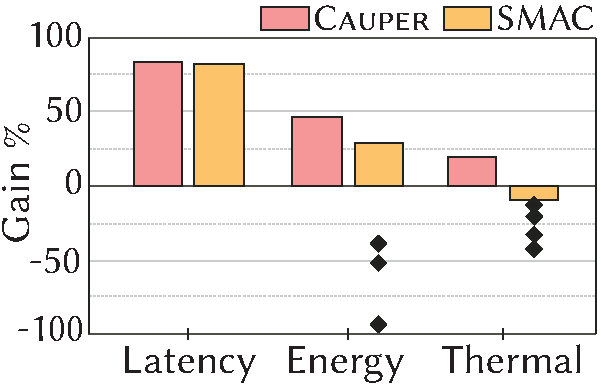
\includegraphics[width=0.3\linewidth]{fig__rq3_a.pdf}
    %     \label{fig:rq3_1_a}
    % }\quad
    \subfloat[Latency]{ \vspace{-1.5em}
        \includegraphics[width=\linewidth]{figures-vg/latency_eff.pdf}
        \label{fig:rq2_1}
    }\\
    \vspace{-1.5em}
    \subfloat[Energy]{
        \includegraphics[width=\linewidth]{figures-vg/energy_eff.pdf}
        \label{fig:rq2_2}
    }
    % \subfloat[Multi Objective]{
    %     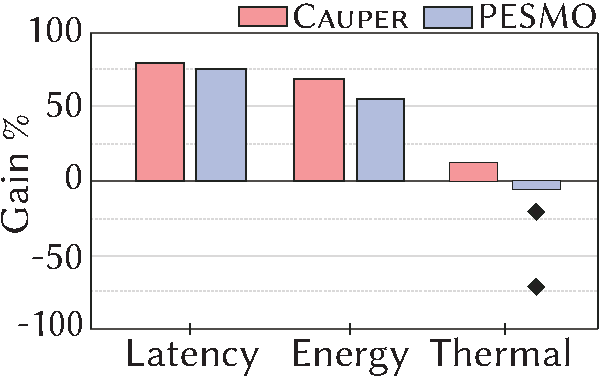
\includegraphics[width=0.275\linewidth]{fig__rq3_b.pdf}
    %     \label{fig:rq3_1_b}
    % }
 
    \caption{\small{\ourapproach has significantly higher sampling efficiency than other baselines in debugging non-functional faults: (a) latency faults in \txtwo and (b) energy faults in \xavier.}}% (indicated by $\blacklozenge$).}}
    \label{tab:rq2_1}
\end{figure}
\noindent{\textbf{Results (debugging).}}~\Cref{tab:single_1,tab:multi_1} shows \ourapproach ~{\em significantly outperforms correlation-based methods in all cases}. For example, in  \textsc{Deepstream} on TX2, \ourapproach achieves 6\% more accuracy, 12\% more precision, and 10\% more recall compared to the next best method, \bugdoc. We observed latency gains as high as $88\%$ ($9\%$ more than \bugdoc) on \txtwo and energy gain of $86\%$ ($9\%$ more than \bugdoc) on \xavier for \textsc{Xception}. We observe similar trends for multi-objective faults as well. The results confirm that \ourapproach~{\em can recommend repairs for faults that significantly improve latency and energy}. By applying the changes to the configurations recommended by \ourapproach improves performance drastically. 


\fig{rq2_1} and \fig{rq2_2} demonstrate the sample efficiency results for different systems. We observe that, for both latency and energy faults, \ourapproach achieved significantly higher gains with substantially fewer samples. For \textsc{Xception}, \ourapproach required a 8$\times$ fewer samples to obtain 32\% higher gain than \textsc{DD}. The higher gain in \ourapproach in comparison to correlation-based methods indicates that \ourapproach's causal reasoning is more effective in guiding the search in the objective space. \ourapproach does not waste budget evaluating configurations with lower causal effects and finds a fix faster.

\begin{figure}[tp!]
    % \subfloat[\tool vs. SMAC for resolving \\latency faults.]{
    %     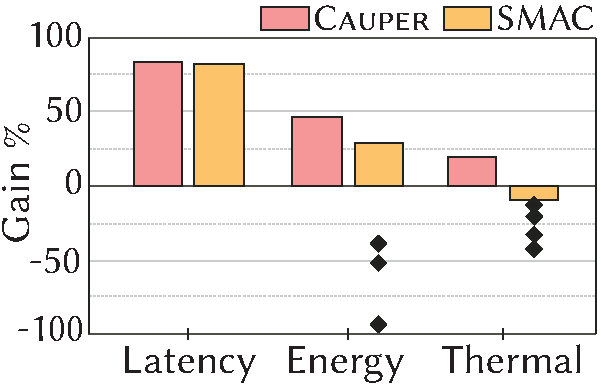
\includegraphics[width=0.3\linewidth]{fig__rq3_a.pdf}
    %     \label{fig:rq3_1_a}
    % }\quad
  
    \includegraphics[width=\linewidth]{figures-vg/sobo_opt_tx2.pdf} 
    \includegraphics[width=\linewidth]{figures-vg/mobo_opt_tx2.pdf}
    \vspace{-4mm}
    \caption{\small{\ourapproach vs. single and multi-objective optimization with SMAC and PESMO in \txtwo.}}% (indicated by $\blacklozenge$).}}
     \label{fig:rq1_opt_se}
    \vspace{-3mm}
\end{figure}

\ourapproach~{\em resolves misconfiguration faults significantly faster than correlation-based approaches}. In~\Cref{tab:single_1,tab:multi_1}, the last two columns indicate the time taken (in hours) by each approach to diagnosing the root cause. For all correlation-based methods, we set a maximum budget of 4 hours. We find that, while other approaches use the entire budget to diagnose and resolve the faults, \ourapproach can do so significantly faster. In particular, we observed that \ourapproach is $13\times$ faster in diagnosing and resolving faults in energy usage for \textsc{x264} deployed on \xavier and $10\times$ faster for latency faults for \textsc{Bert} deployed on \txtwo. 

% All the methods found it difficult to discover the root cause of thermal faults. While \tool outperforms other methods, the overall accuracy, precision, recall, and $\Delta_{gain}$ were lower than corresponding values for latency and energy consumption faults. This is because we performed thermal measurements in a controlled environment to prevent thermal throttling the variance in the measurements was relatively lower than latency and energy consumption.



% \noindent \textbf{Task2. Optimization}
% Here, we employ the learned SCM~\rayb{What is SCM?} as the surrogate model and causal reasoning of effect estimation as the acquisition function for effective exploration of the search space. Mechanisms of counterfactual query evaluation and intervention provide the necessary exploration-exploitation tradeoff.
% The first two phases of \tool is the same as the debugging non-functional fault task. In Phase-III, we use the following queries for single-objective optimization of latency or energy: "\textit{How to improve latency/energy from the optimal so far?}". \tool can natively accommodate multi-objective optimization by slightly altering the counterfactual query. For multi-objective latency and/or energy fault we use the following query: "\textit{How to improve latency or energy by from the optimal observed so far?}". We continue incremental learning until no new configurations are found or the maximum budget of 4 hours is exhausted, whichever occurs first, and return the configuration with minimum latency or energy obtained thus far.

% \noindent \textbf{Setting.}
% For single-objective optimization, we compare \tool with SMAC in \txtwo for \textsc{Xception} for both latency and energy. For multi-objective optimization, PESMO~\cite{hernandez2016predictive} to find a configuration that optimizes for energy and latency simultaneously. We repeat the entire process 3 times for consistent analyses.

% Out of 21 latency faults in image recognition on \txtwo, we found 7 cases (33\%) where the near-optimal configuration caused a significant deterioration in energy consumption. In one case the optimal configuration increased the energy consumption by $96\%$! 
% \noindent\textit{$\circ$~Why \tool works better?}~
% \tool never deteriorates any non-functional property. This is a desirable benefit of using causal graphs. For example, if \tool notices that a configuration option (say) \texttt{GPU frequency} affects both latency and energy consumption, \tool would not recommend changing \texttt{GPU  frequency} to the extent where it consumes too much energy. By design, \tool would explore the possibility of changing other configuration options to improve latency. Optimization approaches are not equipped to handle this. 
 %Note that, while PESMO did not find a configuration that caused high energy consumption, it still suffered from deterioration in heat dissipation in two cases. 


\noindent\textbf{Results (optimization).}~\fig{rq1_opt_se}(a) and \fig{rq1_opt_se}(b) demonstrate the single-objective optimization results---\ourapproach finds configurations with optimal latency and energy for both cases. \fig{rq1_opt_se}(a)  illustrates that the optimal configuration discovered by \ourapproach has 43\% lower latency (12 seconds) than that of SMAC (21 seconds). Here, \ourapproach reaches near-optimal configuration by only exhausting one-third of the entire budget. In \fig{rq1_opt_se}(b), the optimal configuration discovered by \ourapproach and SMAC had almost the same energy, but \ourapproach reached this optimal configuration 4x faster than SMAC. In both single-objective optimizations, the iterative variation of \ourapproach is less than SMAC--i.e., \ourapproach finds more stable configurations. \fig{rq1_opt_se}(c) compares \ourapproach with PESMO to optimize both latency and energy in \txtwo (for image recognition). Here, \ourapproach has 12\% lower hypervolume error than  PESMO and reaches the same level of hypervolume error of PESMO 4x times faster. \fig{rq1_opt_se}(d) illustrates the Pareto optimal configurations obtained by \ourapproach and PESMO. The Pareto front discovered by \ourapproach has higher coverage, as it discovers a larger number of Pareto optimal configurations with lower energy and latency value than PESMO.

% \noindent{\textbf{Discussion.}}~Correlation-based methods rely only on correlation, and this can be misleading since they cannot incorporate the intrinsic complex causal structure of the underlying configuration space. In contrast, \tool relies on causal inference (instead of correlation) to model the configuration space thereby overcoming the limitations with current correlation-based models. Correlation-based methods require a large number of initial observational data for training. They spend most of their allocated 4-hour budget on gathering these training samples. In contrast, \tool starts with only 25 samples and uses incremental learning (\tion{incremental_learning}) to judiciously update the casual graph with better samples that capture the relationships in the search space better. 

%ML-based methods require a large number of initial observational data for training. They expend most of their allocated 4-hour budget on gathering these training samples. In contrast, \tool starts with only 25 samples and uses incremental learning (\tion{incremental_learning}) to judiciously update the casual graph with new configurations until a repair has been found. This drastically reduces the inference time.% and also improves diagnostic capability. %Further, the incremental learning  

% {\em Default configurations perform poorly:} An alternate approach to finding root-cause of a non-functional fault is to compare which configurations in non-functional fault differed from the default configuration. Doing so results in poor performance. The accuracy, precision, and recall were often less than 50\%.


% {\em The cases where CBI is better than} \tool:~
% In one case, with BERT (NLP), deployed on TX2, CBI performs slightly better than \tool, \ie, CBI achieves an accuracy of 68\% and recall of 69\% whereas \tool achieves an accuracy of 64\% and recall of 62\%. However, this comes at a cost of lower precision (57\% in CBI vs. 77\% in \tool); this indicates that CBI detects a large number of false positives. False positives can be detrimental to improving performance. Specifically, for the same case of BERT$\longrightarrow$TX2 in~\tab{rq1_2}, we see that \tool recommends more useful repairs than CBI, \ie, \tool gives us a performance gain of $96\%$ compared to only $76\%$ from CBI.
% \ei
% \noindent\textbf{Why \tool works better?}
% % In general, our results highlight the usefulness of causal models and counterfactual inference that differentiate them from ML-based approaches. 
% \tool uses a causal model to express the complex relationships between configurations and performance and uses this to diagnose the root cause of non-functional faults. Further, using counterfactual inference over the causal model, \tool can recommend useful fixes using only the current observational data. ML-based approaches are limited in this respect. They fail to model the complex interactions between various configuration options and they can only use the observational data provided to them to draw their inferences. They require additional data to build reliable models. This can be both expensive and time-consuming. %In contrast, \tool uses incremental learning 

% \noindent{\textbf{RQ1-B. How effective is \tool in diagnosing multi-objective faults?}}
% 
% %  \begin{table}[]
%      \centering
%      \caption{\small (RQ2) Efficiency of \tool in detecting and repairing the root-cause of multiple non-functional faults. Cells highlighted in \colorbox{blue!10}{green} indicate better performance and \colorbox[HTML]{FFCCC9}{red} indicate cases where the performance drops. Note: the results are reported for two kinds of faults in TX2: (1) faults in both latency and energy; and (2) faults in latency, energy, and heat dissipation.}
%      \label{tab:rq2}
%      \resizebox{\linewidth}{!}{
%      \begin{tabular}{ll|rr|rr|rr|}
%       &  & \multicolumn{1}{r|}{\rotatebox{90}{\tool}} & \rotatebox{90}{Default} & \multicolumn{1}{r|}{\rotatebox{90}{\tool}} & \rotatebox{90}{Default} & \multicolumn{1}{r|}{\rotatebox{90}{\tool}} & \multicolumn{1}{r|}{\rotatebox{90}{Default}} \bigstrut\\ \cline{3-8} 
%       & Software & \multicolumn{2}{r|}{Accuracy} & \multicolumn{2}{r|}{Recall} & \multicolumn{2}{r|}{Precision} \bigstrut\\ \hlineB{2}
%      \multicolumn{1}{l|}{\multirow{6.5}{*}{Latency and Energy}} & DNN Image & \cellcolor{blue!10}59 & 51 & \cellcolor{blue!10}44 & 35 & \cellcolor{blue!10}65 & 56 \bigstrut\\
%      \multicolumn{1}{l|}{} & DNN   Speech & \cellcolor{blue!10}66 & 49 & \cellcolor{blue!10}51 & 43 & \cellcolor{blue!10}74 & 64 \bigstrut\\
%      \multicolumn{1}{l|}{} & DNN NLP & \cellcolor{blue!10}56 & 53 & \cellcolor{blue!10}42 & \cellcolor{blue!10}42 & \cellcolor{blue!10}66 & 61 \bigstrut\\
%      \multicolumn{1}{l|}{} & x264 & \cellcolor{blue!10}51 & 48 & \cellcolor{blue!10}55 & 33 & \cellcolor{blue!10}64 & 56 \bigstrut\\
%      \multicolumn{1}{l|}{} & SQLite & \cellcolor{blue!10}60 & 51 & \cellcolor{blue!10}57 & 37 & \cellcolor{blue!10}72 & 57 \bigstrut\\ \hlineB{2}
%      \multicolumn{1}{l|}{\multirow{3}{*}{All three}} & DNN Image & \cellcolor{blue!10}67 & 59 & \cellcolor{blue!10}69 & 60 & \cellcolor{blue!10}64 & 60 \bigstrut\\
%      \multicolumn{1}{l|}{} & x264 & \cellcolor{blue!10}68 & 62 & \cellcolor{blue!10}79 & 56 & \cellcolor{blue!10}68 & 58 \bigstrut\\
%      \multicolumn{1}{l|}{} & SQLite & \cellcolor{blue!10}79 & 63 & \cellcolor{blue!10}70 & 57 & \cellcolor{blue!10}84 & 63 \bigstrut\\ \hlineB{2}\multicolumn{1}{l}{}&\multicolumn{1}{l}{}&\multicolumn{1}{l}{}&\multicolumn{1}{l}{}&\multicolumn{1}{l}{}&\multicolumn{1}{l}{}&\multicolumn{1}{l}{}\bigstrut\\[-0.4cm]\hlineB{2}
%      \multicolumn{1}{l}{\multirow{9.5}{*}{Latency and Energy}} & \multicolumn{1}{r|}{$\Delta_{gain}\longrightarrow$} & \multicolumn{2}{c|}{{Latency}} & \multicolumn{2}{c|}{{Energy}} & \multicolumn{2}{c|}{{Thermals}} \bigstrut\\ \hlineB{2} 
    
%      \multicolumn{1}{l|}{} & DNN Image & \cellcolor{blue!10}52 & \multicolumn{1}{l|}{33} & \multicolumn{1}{l}{\cellcolor{blue!10}37} & \multicolumn{1}{l|}{22} & \multicolumn{1}{l}{0} & \multicolumn{1}{l|}{0} \bigstrut\\
    
%      \multicolumn{1}{l|}{} & DNN   Speech & \multicolumn{1}{l}{\cellcolor{blue!10}60} & \multicolumn{1}{l|}{25} & \multicolumn{1}{l}{\cellcolor{blue!10}54} & \multicolumn{1}{l|}{17} & \multicolumn{1}{l}{0} & \multicolumn{1}{l|}{0} \bigstrut\\
    
%      \multicolumn{1}{l|}{} & DNN NLP & \multicolumn{1}{l}{\cellcolor{blue!10}49} & \multicolumn{1}{l|}{30} & \multicolumn{1}{l}{\cellcolor{blue!10}51} & \multicolumn{1}{l|}{17} & \multicolumn{1}{l}{0} & \multicolumn{1}{l|}{0} \bigstrut\\
    
%      \multicolumn{1}{l|}{} & x264 & \multicolumn{1}{l}{\cellcolor{blue!10}23} & \multicolumn{1}{l|}{2} & \multicolumn{1}{l}{\cellcolor{blue!10}12} & \multicolumn{1}{l|}{\cellcolor[HTML]{FFCCC9}-2} & \multicolumn{1}{l}{0} & \multicolumn{1}{l|}{\cellcolor[HTML]{FFCCC9}-1} \bigstrut\\
    
%      \multicolumn{1}{l|}{} & SQLite & \multicolumn{1}{l}{\cellcolor{blue!10}9} & \multicolumn{1}{l|}{6} & \multicolumn{1}{l}{\cellcolor{blue!10}11} & \multicolumn{1}{l|}{2} & \multicolumn{1}{l}{0} & \multicolumn{1}{l|}{\cellcolor[HTML]{FFCCC9}-1} \bigstrut\\ \hlineB{2}
    
%      \multicolumn{1}{l|}{\multirow{3}{*}{All three}} & DNN Image & \multicolumn{1}{l}{\cellcolor{blue!10}54} & \multicolumn{1}{l|}{29} & \multicolumn{1}{l}{\cellcolor{blue!10}31} & \multicolumn{1}{l|}{16} & \multicolumn{1}{l}{1} & \multicolumn{1}{l|}{1} \bigstrut\\
    
%      \multicolumn{1}{l|}{} & x264 & \multicolumn{1}{l}{\cellcolor{blue!10}18} & \multicolumn{1}{l|}{1} & \multicolumn{1}{l}{\cellcolor{blue!10}10} & \multicolumn{1}{l|}{\cellcolor[HTML]{FFCCC9}-1} & \multicolumn{1}{l}{1} & \multicolumn{1}{l|}{\cellcolor[HTML]{FFCCC9}-1} \bigstrut\\
   
%      \multicolumn{1}{l|}{} & SQLite & \multicolumn{1}{l}{\cellcolor{blue!10}6} & \multicolumn{1}{l|}{3} & \multicolumn{1}{l}{\cellcolor{blue!10}7} & \multicolumn{1}{l|}{2} & \multicolumn{1}{l}{1} & \multicolumn{1}{l|}{0} \bigstrut\\ \hlineB{2}
%      \end{tabular}
%      }
%      \end{table}

\begin{table*}[]
    \centering
    \caption{\small {Efficiency of \tool in detecting and repairing the root-cause of multiple non-functional faults: \textit{Energy, Latency}; and \textit{Energy, Latency, Heat}. Cells highlighted in \colorbox{blue!10}{green} indicate improvement over faults and \colorbox[HTML]{FFCCC9}{red} indicate deterioration. \tool achieves better performance overall and is much faster. Note: the results are reported for NVIDIA Jetson TX2.}}
    \label{tab:rq2}
    \footnotesize
    \resizebox{\textwidth}{!}{
        \begin{tabular}{@{}l@{}ll|llll|llll|llll|llll|llll|llll|ll|}
            \clineB{4-29}{2}
            &  &  & \multicolumn{4}{c|}{Accuracy} & \multicolumn{4}{c|}{Precision} & \multicolumn{4}{c|}{Recall} & \multicolumn{4}{c|}{Gain (Latency)} & \multicolumn{4}{c|}{Gain (Energy)} & \multicolumn{4}{c|}{Gain (Heat)} & \multicolumn{2}{c|}{Time$^\dagger$} \bigstrut\\ \clineB{4-29}{2}
            % &  &  &  &  &  &  &  &  & \\[-1em]\clineB{4-29}{2} 
            
            &  &  & \rotatebox{90}{\bfseries\tool~} & \rotatebox{90}{\cbi} & \rotatebox{90}{\encore} & \rotatebox{90}{\bugdoc} & \rotatebox{90}{\bfseries\tool~} & \rotatebox{90}{\cbi} & \rotatebox{90}{\encore} & \rotatebox{90}{\bugdoc} & \rotatebox{90}{\bfseries\tool~} & \rotatebox{90}{\cbi} & \rotatebox{90}{\encore} & \rotatebox{90}{\bugdoc} & \rotatebox{90}{\bfseries\tool~} & \rotatebox{90}{\cbi} & \rotatebox{90}{\encore} & \rotatebox{90}{\bugdoc} & \rotatebox{90}{\bfseries\tool~} & \rotatebox{90}{\cbi} & \rotatebox{90}{\encore} & \rotatebox{90}{\bugdoc} & \rotatebox{90}{\bfseries\tool~} & \rotatebox{90}{\cbi} & \rotatebox{90}{\encore} & \rotatebox{90}{\bugdoc} & \rotatebox{90}{\bfseries\tool~} & \rotatebox{90}{Others} \\ \clineB{4-29}{2}
            
            \multicolumn{1}{l}{}&\multicolumn{1}{l}{}  & \multicolumn{1}{l}{} & \multicolumn{1}{l}{} & \multicolumn{1}{l}{} & \multicolumn{1}{l}{} & \multicolumn{1}{l}{} & \multicolumn{1}{l}{} & \multicolumn{1}{l}{} & \multicolumn{1}{l}{} \\[-0.9em]\hlineB{2}

            & \multicolumn{1}{l|}{} & Image & \cellcolor{blue!10}\textbf{77} & 54 & 55 & 65 & \cellcolor{blue!10}\textbf{73} & 53 & 54 & 62 & \cellcolor{blue!10}\textbf{80} & 59 & 59 & 62 & \cellcolor{blue!10}\textbf{83} & 53 & 61 & 65 & \cellcolor{blue!10}\textbf{70} & 38 & 46 & 44 & \cellcolor{blue!10}\textbf{3} & 0 & 0 & 0 & \cellcolor{blue!10}\textbf{0.6} & 4 \\
            & \multicolumn{1}{l|}{} & NLP & \cellcolor{blue!10}\textbf{70} & 51 & 56 & 65 & \cellcolor{blue!10}\textbf{71} & 42 & 56 & 63 & \cellcolor{blue!10}\textbf{66} & 59 & 62 & 65 & \cellcolor{blue!10}\textbf{68} & 53 & 59 & 61 & \cellcolor{blue!10}\textbf{60} & 41 & 27 & 48 & \cellcolor{blue!10}\textbf{5} & 0 & 0 & 1 & \cellcolor{blue!10}\textbf{0.2} & 4 \\
            & \multicolumn{1}{l|}{} & Speech & \cellcolor{blue!10}\textbf{74} & 50 & 61 & 65 & \cellcolor{blue!10}\textbf{68} & 44 & 53 & 62 & \cellcolor{blue!10}\textbf{79} & 51 & 59 & 64 & \cellcolor{blue!10}\textbf{82} & 55 & 55 & 62 & \cellcolor{blue!10}\textbf{66} & 43 & 43 & 41 & \cellcolor{blue!10}\textbf{4} & \cellcolor[HTML]{FFCCC9}-2 & \cellcolor[HTML]{FFCCC9}-1 & \cellcolor[HTML]{FFCCC9}-1 & \cellcolor{blue!10}\textbf{0.7} & 4 \\
            & \multicolumn{1}{l|}{} & x264 & \cellcolor{blue!10}\textbf{83} & 54 & 55 & 66 & \cellcolor{blue!10}\textbf{81} & 50 & 54 & 57 & \cellcolor{blue!10}\textbf{77} & 63 & 62 & 61 & \cellcolor{blue!10}\textbf{15} & 2 & 4 & 6 & \cellcolor{blue!10}\textbf{13} & 4 & 6 & 4 & \cellcolor{blue!10}\textbf{2} & \cellcolor[HTML]{FFCCC9}-3 & \cellcolor[HTML]{FFCCC9}-1 & 0 & \cellcolor{blue!10}\textbf{1.2} & 4 \\
           \multirow{-5}{*}{\rotatebox{90}{Energy +}} & \multicolumn{1}{l|}{\multirow{-5}{*}{\rotatebox{90}{Latency}}} & SQLite & \cellcolor{blue!10}\textbf{84} & 51 & 58 & 68 & \cellcolor{blue!10}\textbf{80} & 43 & 55 & 62 & \cellcolor{blue!10}\textbf{84} & 57 & 63 & 65 & \cellcolor{blue!10}\textbf{11} & 5 & 4 & 5 & \cellcolor{blue!10}\textbf{14} & 3 & 8 & 8 & \cellcolor{blue!10}\textbf{2} & \cellcolor[HTML]{FFCCC9}-2 & 0 & \cellcolor[HTML]{FFCCC9}-1 & \cellcolor{blue!10}\textbf{0.5} & 4 \\ \hlineB{2}

           \multicolumn{1}{l}{}&\multicolumn{1}{l}{}  & \multicolumn{1}{l}{} & \multicolumn{1}{l}{} & \multicolumn{1}{l}{} & \multicolumn{1}{l}{} & \multicolumn{1}{l}{} & \multicolumn{1}{l}{} & \multicolumn{1}{l}{} & \multicolumn{1}{l}{} \\[-0.95em]\hlineB{2}

            & \multicolumn{1}{l|}{} & Image & \cellcolor{blue!10}\textbf{76} & 57 & 48 & 66 & \cellcolor{blue!10}\textbf{68} & 61 & 57 & 61 & \cellcolor{blue!10}\textbf{81} & 53 & 46 & 70 & \cellcolor{blue!10}\textbf{62} & 33 & 30 & 42 & \cellcolor{blue!10}\textbf{52} & 23 & 18 & 24 & \cellcolor{blue!10}\textbf{4} & 1 & 0 & 0 & \cellcolor{blue!10}\textbf{0.1} & 4 \\
            & \multicolumn{1}{l|}{} & x264 & \cellcolor{blue!10}\textbf{80} & 59 & 47 & 54 & \cellcolor{blue!10}\textbf{76} & 61 & 56 & 63 & \cellcolor{blue!10}\textbf{81} & 56 & 46 & 51 & \cellcolor{blue!10}\textbf{12} & 2 & 1 & 2 & \cellcolor{blue!10}\textbf{15} & 4 & 2 & 4 & \cellcolor{blue!10}\textbf{4} & 1 & 0 & 1 & \cellcolor{blue!10}\textbf{0.1} & 4 \\
           \multirow{-3}{*}{\rotatebox{90}{All}} & \multicolumn{1}{l|}{\multirow{-3}{*}{\rotatebox{90}{Three}}} & SQLite & \cellcolor{blue!10}\textbf{73} & 56 & 51 & 53 & \cellcolor{blue!10}\textbf{68} & 59 & 56 & 60 & \cellcolor{blue!10}\textbf{78} & 54 & 45 & 51 & \cellcolor{blue!10}\textbf{12} & 1 & 1 & 4 & \cellcolor{blue!10}\textbf{8} & 4 & 2 & 5 & \cellcolor{blue!10}\textbf{1} & 1 & \cellcolor[HTML]{FFCCC9}-1 & \cellcolor[HTML]{FFCCC9}-1 & \cellcolor{blue!10}\textbf{0.1} & 4 \\ \hlineB{2}
           \multicolumn{10}{l}{$^\dagger$ Wallclock time in hours}\bigstrut
           \end{tabular}
    }
\end{table*}
    
% This RQ focuses on multi-objective faults where misconfigurations affect multiple non-functional properties simultaneously, \ie, in latency \textit{and} energy consumption. %In this section, 
% we emulate the scenario where a user experiences such multi-objective faults and uses \tool to help answer the following two questions:
% \bi[leftmargin=*]
% \item What is the root cause of my non-functional fault? 
% \item What can I change to repair my performance on the faulty objectives while not degrading the correctly functioning objectives?
% \ei
% Similar to RQ1, 
% we evaluate how well \tool can diagnose and fix such faults.
% 
% %  \begin{table}[]
%      \centering
%      \caption{\small (RQ2) Efficiency of \tool in detecting and repairing the root-cause of multiple non-functional faults. Cells highlighted in \colorbox{blue!10}{green} indicate better performance and \colorbox[HTML]{FFCCC9}{red} indicate cases where the performance drops. Note: the results are reported for two kinds of faults in TX2: (1) faults in both latency and energy; and (2) faults in latency, energy, and heat dissipation.}
%      \label{tab:rq2}
%      \resizebox{\linewidth}{!}{
%      \begin{tabular}{ll|rr|rr|rr|}
%       &  & \multicolumn{1}{r|}{\rotatebox{90}{\tool}} & \rotatebox{90}{Default} & \multicolumn{1}{r|}{\rotatebox{90}{\tool}} & \rotatebox{90}{Default} & \multicolumn{1}{r|}{\rotatebox{90}{\tool}} & \multicolumn{1}{r|}{\rotatebox{90}{Default}} \bigstrut\\ \cline{3-8} 
%       & Software & \multicolumn{2}{r|}{Accuracy} & \multicolumn{2}{r|}{Recall} & \multicolumn{2}{r|}{Precision} \bigstrut\\ \hlineB{2}
%      \multicolumn{1}{l|}{\multirow{6.5}{*}{Latency and Energy}} & DNN Image & \cellcolor{blue!10}59 & 51 & \cellcolor{blue!10}44 & 35 & \cellcolor{blue!10}65 & 56 \bigstrut\\
%      \multicolumn{1}{l|}{} & DNN   Speech & \cellcolor{blue!10}66 & 49 & \cellcolor{blue!10}51 & 43 & \cellcolor{blue!10}74 & 64 \bigstrut\\
%      \multicolumn{1}{l|}{} & DNN NLP & \cellcolor{blue!10}56 & 53 & \cellcolor{blue!10}42 & \cellcolor{blue!10}42 & \cellcolor{blue!10}66 & 61 \bigstrut\\
%      \multicolumn{1}{l|}{} & x264 & \cellcolor{blue!10}51 & 48 & \cellcolor{blue!10}55 & 33 & \cellcolor{blue!10}64 & 56 \bigstrut\\
%      \multicolumn{1}{l|}{} & SQLite & \cellcolor{blue!10}60 & 51 & \cellcolor{blue!10}57 & 37 & \cellcolor{blue!10}72 & 57 \bigstrut\\ \hlineB{2}
%      \multicolumn{1}{l|}{\multirow{3}{*}{All three}} & DNN Image & \cellcolor{blue!10}67 & 59 & \cellcolor{blue!10}69 & 60 & \cellcolor{blue!10}64 & 60 \bigstrut\\
%      \multicolumn{1}{l|}{} & x264 & \cellcolor{blue!10}68 & 62 & \cellcolor{blue!10}79 & 56 & \cellcolor{blue!10}68 & 58 \bigstrut\\
%      \multicolumn{1}{l|}{} & SQLite & \cellcolor{blue!10}79 & 63 & \cellcolor{blue!10}70 & 57 & \cellcolor{blue!10}84 & 63 \bigstrut\\ \hlineB{2}\multicolumn{1}{l}{}&\multicolumn{1}{l}{}&\multicolumn{1}{l}{}&\multicolumn{1}{l}{}&\multicolumn{1}{l}{}&\multicolumn{1}{l}{}&\multicolumn{1}{l}{}\bigstrut\\[-0.4cm]\hlineB{2}
%      \multicolumn{1}{l}{\multirow{9.5}{*}{Latency and Energy}} & \multicolumn{1}{r|}{$\Delta_{gain}\longrightarrow$} & \multicolumn{2}{c|}{{Latency}} & \multicolumn{2}{c|}{{Energy}} & \multicolumn{2}{c|}{{Thermals}} \bigstrut\\ \hlineB{2} 
    
%      \multicolumn{1}{l|}{} & DNN Image & \cellcolor{blue!10}52 & \multicolumn{1}{l|}{33} & \multicolumn{1}{l}{\cellcolor{blue!10}37} & \multicolumn{1}{l|}{22} & \multicolumn{1}{l}{0} & \multicolumn{1}{l|}{0} \bigstrut\\
    
%      \multicolumn{1}{l|}{} & DNN   Speech & \multicolumn{1}{l}{\cellcolor{blue!10}60} & \multicolumn{1}{l|}{25} & \multicolumn{1}{l}{\cellcolor{blue!10}54} & \multicolumn{1}{l|}{17} & \multicolumn{1}{l}{0} & \multicolumn{1}{l|}{0} \bigstrut\\
    
%      \multicolumn{1}{l|}{} & DNN NLP & \multicolumn{1}{l}{\cellcolor{blue!10}49} & \multicolumn{1}{l|}{30} & \multicolumn{1}{l}{\cellcolor{blue!10}51} & \multicolumn{1}{l|}{17} & \multicolumn{1}{l}{0} & \multicolumn{1}{l|}{0} \bigstrut\\
    
%      \multicolumn{1}{l|}{} & x264 & \multicolumn{1}{l}{\cellcolor{blue!10}23} & \multicolumn{1}{l|}{2} & \multicolumn{1}{l}{\cellcolor{blue!10}12} & \multicolumn{1}{l|}{\cellcolor[HTML]{FFCCC9}-2} & \multicolumn{1}{l}{0} & \multicolumn{1}{l|}{\cellcolor[HTML]{FFCCC9}-1} \bigstrut\\
    
%      \multicolumn{1}{l|}{} & SQLite & \multicolumn{1}{l}{\cellcolor{blue!10}9} & \multicolumn{1}{l|}{6} & \multicolumn{1}{l}{\cellcolor{blue!10}11} & \multicolumn{1}{l|}{2} & \multicolumn{1}{l}{0} & \multicolumn{1}{l|}{\cellcolor[HTML]{FFCCC9}-1} \bigstrut\\ \hlineB{2}
    
%      \multicolumn{1}{l|}{\multirow{3}{*}{All three}} & DNN Image & \multicolumn{1}{l}{\cellcolor{blue!10}54} & \multicolumn{1}{l|}{29} & \multicolumn{1}{l}{\cellcolor{blue!10}31} & \multicolumn{1}{l|}{16} & \multicolumn{1}{l}{1} & \multicolumn{1}{l|}{1} \bigstrut\\
    
%      \multicolumn{1}{l|}{} & x264 & \multicolumn{1}{l}{\cellcolor{blue!10}18} & \multicolumn{1}{l|}{1} & \multicolumn{1}{l}{\cellcolor{blue!10}10} & \multicolumn{1}{l|}{\cellcolor[HTML]{FFCCC9}-1} & \multicolumn{1}{l}{1} & \multicolumn{1}{l|}{\cellcolor[HTML]{FFCCC9}-1} \bigstrut\\
   
%      \multicolumn{1}{l|}{} & SQLite & \multicolumn{1}{l}{\cellcolor{blue!10}6} & \multicolumn{1}{l|}{3} & \multicolumn{1}{l}{\cellcolor{blue!10}7} & \multicolumn{1}{l|}{2} & \multicolumn{1}{l}{1} & \multicolumn{1}{l|}{0} \bigstrut\\ \hlineB{2}
%      \end{tabular}
%      }
%      \end{table}

\begin{table*}[]
    \centering
    \caption{\small {Efficiency of \tool in detecting and repairing the root-cause of multiple non-functional faults: \textit{Energy, Latency}; and \textit{Energy, Latency, Heat}. Cells highlighted in \colorbox{blue!10}{green} indicate improvement over faults and \colorbox[HTML]{FFCCC9}{red} indicate deterioration. \tool achieves better performance overall and is much faster. Note: the results are reported for NVIDIA Jetson TX2.}}
    \label{tab:rq2}
    \footnotesize
    \resizebox{\textwidth}{!}{
        \begin{tabular}{@{}l@{}ll|llll|llll|llll|llll|llll|llll|ll|}
            \clineB{4-29}{2}
            &  &  & \multicolumn{4}{c|}{Accuracy} & \multicolumn{4}{c|}{Precision} & \multicolumn{4}{c|}{Recall} & \multicolumn{4}{c|}{Gain (Latency)} & \multicolumn{4}{c|}{Gain (Energy)} & \multicolumn{4}{c|}{Gain (Heat)} & \multicolumn{2}{c|}{Time$^\dagger$} \bigstrut\\ \clineB{4-29}{2}
            % &  &  &  &  &  &  &  &  & \\[-1em]\clineB{4-29}{2} 
            
            &  &  & \rotatebox{90}{\bfseries\tool~} & \rotatebox{90}{\cbi} & \rotatebox{90}{\encore} & \rotatebox{90}{\bugdoc} & \rotatebox{90}{\bfseries\tool~} & \rotatebox{90}{\cbi} & \rotatebox{90}{\encore} & \rotatebox{90}{\bugdoc} & \rotatebox{90}{\bfseries\tool~} & \rotatebox{90}{\cbi} & \rotatebox{90}{\encore} & \rotatebox{90}{\bugdoc} & \rotatebox{90}{\bfseries\tool~} & \rotatebox{90}{\cbi} & \rotatebox{90}{\encore} & \rotatebox{90}{\bugdoc} & \rotatebox{90}{\bfseries\tool~} & \rotatebox{90}{\cbi} & \rotatebox{90}{\encore} & \rotatebox{90}{\bugdoc} & \rotatebox{90}{\bfseries\tool~} & \rotatebox{90}{\cbi} & \rotatebox{90}{\encore} & \rotatebox{90}{\bugdoc} & \rotatebox{90}{\bfseries\tool~} & \rotatebox{90}{Others} \\ \clineB{4-29}{2}
            
            \multicolumn{1}{l}{}&\multicolumn{1}{l}{}  & \multicolumn{1}{l}{} & \multicolumn{1}{l}{} & \multicolumn{1}{l}{} & \multicolumn{1}{l}{} & \multicolumn{1}{l}{} & \multicolumn{1}{l}{} & \multicolumn{1}{l}{} & \multicolumn{1}{l}{} \\[-0.9em]\hlineB{2}

            & \multicolumn{1}{l|}{} & Image & \cellcolor{blue!10}\textbf{77} & 54 & 55 & 65 & \cellcolor{blue!10}\textbf{73} & 53 & 54 & 62 & \cellcolor{blue!10}\textbf{80} & 59 & 59 & 62 & \cellcolor{blue!10}\textbf{83} & 53 & 61 & 65 & \cellcolor{blue!10}\textbf{70} & 38 & 46 & 44 & \cellcolor{blue!10}\textbf{3} & 0 & 0 & 0 & \cellcolor{blue!10}\textbf{0.6} & 4 \\
            & \multicolumn{1}{l|}{} & NLP & \cellcolor{blue!10}\textbf{70} & 51 & 56 & 65 & \cellcolor{blue!10}\textbf{71} & 42 & 56 & 63 & \cellcolor{blue!10}\textbf{66} & 59 & 62 & 65 & \cellcolor{blue!10}\textbf{68} & 53 & 59 & 61 & \cellcolor{blue!10}\textbf{60} & 41 & 27 & 48 & \cellcolor{blue!10}\textbf{5} & 0 & 0 & 1 & \cellcolor{blue!10}\textbf{0.2} & 4 \\
            & \multicolumn{1}{l|}{} & Speech & \cellcolor{blue!10}\textbf{74} & 50 & 61 & 65 & \cellcolor{blue!10}\textbf{68} & 44 & 53 & 62 & \cellcolor{blue!10}\textbf{79} & 51 & 59 & 64 & \cellcolor{blue!10}\textbf{82} & 55 & 55 & 62 & \cellcolor{blue!10}\textbf{66} & 43 & 43 & 41 & \cellcolor{blue!10}\textbf{4} & \cellcolor[HTML]{FFCCC9}-2 & \cellcolor[HTML]{FFCCC9}-1 & \cellcolor[HTML]{FFCCC9}-1 & \cellcolor{blue!10}\textbf{0.7} & 4 \\
            & \multicolumn{1}{l|}{} & x264 & \cellcolor{blue!10}\textbf{83} & 54 & 55 & 66 & \cellcolor{blue!10}\textbf{81} & 50 & 54 & 57 & \cellcolor{blue!10}\textbf{77} & 63 & 62 & 61 & \cellcolor{blue!10}\textbf{15} & 2 & 4 & 6 & \cellcolor{blue!10}\textbf{13} & 4 & 6 & 4 & \cellcolor{blue!10}\textbf{2} & \cellcolor[HTML]{FFCCC9}-3 & \cellcolor[HTML]{FFCCC9}-1 & 0 & \cellcolor{blue!10}\textbf{1.2} & 4 \\
           \multirow{-5}{*}{\rotatebox{90}{Energy +}} & \multicolumn{1}{l|}{\multirow{-5}{*}{\rotatebox{90}{Latency}}} & SQLite & \cellcolor{blue!10}\textbf{84} & 51 & 58 & 68 & \cellcolor{blue!10}\textbf{80} & 43 & 55 & 62 & \cellcolor{blue!10}\textbf{84} & 57 & 63 & 65 & \cellcolor{blue!10}\textbf{11} & 5 & 4 & 5 & \cellcolor{blue!10}\textbf{14} & 3 & 8 & 8 & \cellcolor{blue!10}\textbf{2} & \cellcolor[HTML]{FFCCC9}-2 & 0 & \cellcolor[HTML]{FFCCC9}-1 & \cellcolor{blue!10}\textbf{0.5} & 4 \\ \hlineB{2}

           \multicolumn{1}{l}{}&\multicolumn{1}{l}{}  & \multicolumn{1}{l}{} & \multicolumn{1}{l}{} & \multicolumn{1}{l}{} & \multicolumn{1}{l}{} & \multicolumn{1}{l}{} & \multicolumn{1}{l}{} & \multicolumn{1}{l}{} & \multicolumn{1}{l}{} \\[-0.95em]\hlineB{2}

            & \multicolumn{1}{l|}{} & Image & \cellcolor{blue!10}\textbf{76} & 57 & 48 & 66 & \cellcolor{blue!10}\textbf{68} & 61 & 57 & 61 & \cellcolor{blue!10}\textbf{81} & 53 & 46 & 70 & \cellcolor{blue!10}\textbf{62} & 33 & 30 & 42 & \cellcolor{blue!10}\textbf{52} & 23 & 18 & 24 & \cellcolor{blue!10}\textbf{4} & 1 & 0 & 0 & \cellcolor{blue!10}\textbf{0.1} & 4 \\
            & \multicolumn{1}{l|}{} & x264 & \cellcolor{blue!10}\textbf{80} & 59 & 47 & 54 & \cellcolor{blue!10}\textbf{76} & 61 & 56 & 63 & \cellcolor{blue!10}\textbf{81} & 56 & 46 & 51 & \cellcolor{blue!10}\textbf{12} & 2 & 1 & 2 & \cellcolor{blue!10}\textbf{15} & 4 & 2 & 4 & \cellcolor{blue!10}\textbf{4} & 1 & 0 & 1 & \cellcolor{blue!10}\textbf{0.1} & 4 \\
           \multirow{-3}{*}{\rotatebox{90}{All}} & \multicolumn{1}{l|}{\multirow{-3}{*}{\rotatebox{90}{Three}}} & SQLite & \cellcolor{blue!10}\textbf{73} & 56 & 51 & 53 & \cellcolor{blue!10}\textbf{68} & 59 & 56 & 60 & \cellcolor{blue!10}\textbf{78} & 54 & 45 & 51 & \cellcolor{blue!10}\textbf{12} & 1 & 1 & 4 & \cellcolor{blue!10}\textbf{8} & 4 & 2 & 5 & \cellcolor{blue!10}\textbf{1} & 1 & \cellcolor[HTML]{FFCCC9}-1 & \cellcolor[HTML]{FFCCC9}-1 & \cellcolor{blue!10}\textbf{0.1} & 4 \\ \hlineB{2}
           \multicolumn{10}{l}{$^\dagger$ Wallclock time in hours}\bigstrut
           \end{tabular}
    }
\end{table*}
    
% \approach  
% ~Similar to the previous section, we seed \tool with 25 initial samples. For other methods, we train with 500 sample configurations and their corresponding latency, energy consumption, and thermal output gathered randomly.
% 
% We report our results for \textit{(Latency, Energy)} faults and \textit{(Latency, Energy)} faults. 
% 
% We chose \txtwo because it was more powerful than \txone and more energy and thermally efficient than \xavier. 
% The findings, reported for \txtwo, are representative of multi-objective non-functional faults all across other software and hardware combinations. %Complete results are available in the \href{https://git.io/JUI61}{replication package}.

% \observations 
% From~\tab{rq2}, we observe the following:

% % tabulates the effectiveness of \tool in identifying the root causes and recommending repairs for multiple non-functional faults. Note: Each cell in \tab{rq2} reports the average, the variance as less than 3\% in all cases.
% %  we present a summary of our findings using multi-objective non-functional faults observed in \txtwo. 
% % txtwo had several multi-objective faults. W\e study two groups of multi-objective non-functional faults: 
% \noindent\textbf{$\bullet~$~\textit{Accuracy, Precision, and Recall.}~}
% In all cases, we find that \tool could diagnose and fix misconfigurations more effectively compared to other approaches. On average, accuracy, precision, and recall of \tool were 15\% higher. %than other methods.  
% % In the best case (Latency-Energy faults in SQLite), \tool can achieve accuracy of up to $84\%$ compared to about $68\%$ when using \bugdoc (the second-best method). %We observe similar trends with precision (\tool achieves $81\%$ in x264 vs. $57\%$ with \bugdoc) and recall (\tool achieves $84\%$ in SQLite vs. $65\%$ with \bugdoc). 

% % \item \textit{Finding root causes for multi-objective non-functional faults is harder than single-objective faults:}~The accuracy, precision, and recall for finding multi-objective non-functional faults were lower than the corresponding values in the single objective scenario. We attribute this to the quality of 

% \noindent\textbf{$\bullet~$~\textit{Gain.}~}
% % The fixes recommended by \tool resolved all the multi-objective faults with significantly better improvement (gain) in latency, energy, and heat dissipation. Specifically, \tool had (on average) $13\%$ higher latency gain, $17\%$ higher energy gain, and 5\% higher thermal gain. 
% % Except for \tool, all other methods lead to a degradation in one or more non-functional properties (highlighted in \colorbox[HTML]{FFCCC9}{red} in~\tab{rq2}). This is a limitation of ML-models; some configuration options have \textit{multiple effects}, \eg, increasing \texttt{core frequency} reduces latency, but it increases energy consumption and also increases heat dissipation (more energy and cooling is required to accommodate higher clock speeds). ML models cannot model such nuances, while the causal model used in \tool can.
% Similar to RQ1-A, we find that \tool could fix misconfigurations more effectively compared to other approaches. Compared to the next best method (\bugdoc) the gain offered by \tool was, on average, 19.25\% higher for latency faults and 24.5\% higher for energy faults.

% % Using default, one would change all the faulty configurations to their default values. While this approach offers marginal performance improvement, the repairs recommended by \tool result in significantly higher performance gain on all the faulty objectives. Further, repairs from \tool do not negatively impact the correct functioning objective. For example, in the case of latency-energy faults in DNN based speech processing applications, repairs from \tool yield a performance improvement of $60\%$ on latency and $54\%$ on energy consumption. In contrast, using the default configuration, we obtain an improvement of only $25\%$ on latency and $17\%$ on energy consumption. 


% \noindent\textbf{$\bullet~$~\textit{Wallclock time.}~}~As with RQ1-A, \tool is, on average, $5\times$ faster than ML-based methods.

% \bi[leftmargin=*]







% \noindent\textit{3. Why does the DNN application offer better gain than x264?}
% \Cref{tab:rq1_1,tab:rq2} shows that, DNN applications had the most improvement with \tool compared to x264. This is because misconfigurations affecting the onboard GPU lead to severe degradation in latency and energy usage. Since DNN relies on GPU to optimize the operations, it must be configured appropriately to leverage the full hardware potential. However, x264 is not affected by GPU misconfigurations.
% \tool could identify these misconfigurations better than ML-based methods.

% \ei 
% In summary, we find that: 

% existing ML-based debugging approaches are not applicable for multi-objective non-functional faults and using a default, albeit common, is not always better. \tool, by design, can learn a causal graph that  
% accommodates multiple objectives. Using specific counterfactual queries over this causal model \tool and recommended useful repairs for faults on more than one of the objectives. 

% \begin{result}
%     \textit{\textbf{Key findings}}
%     \bisq
%     \item \tool is more effective than ML-based in diagnostics approaches in mitigating multiple non-functional faults.
%     \item Unlike \tool, ML-based approaches can result in deterioration in one or more non-functional properties.
%     \item \tool is much faster (avg. $9\times$) than other approaches.
%     \ei
% \end{result}

% \begin{result}
% % \textbf{Summary.}~
% \tool outperforms ML-based approaches in detecting diagnosing and mitigating both single- and multi-objective \nfps with gains of up to $34\%$ greater than the next best method. \tool is also $2.8\times-10\times$ faster than other approaches.     
% \end{result}








% \begin{figure}
%     \setlength{\belowcaptionskip}{-2em}
%     \subfloat[Sensitivity to workload change.]{
%     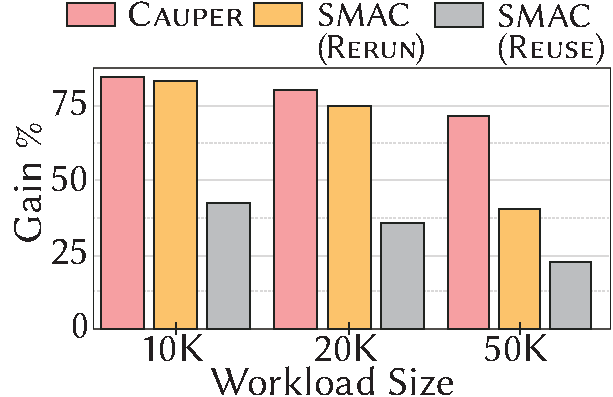
\includegraphics[width=0.45\linewidth]{fig__rq3_d.pdf}
%     \label{fig:rq3_2_a}
%     }~
%     \subfloat[Wallclock time.]{
%         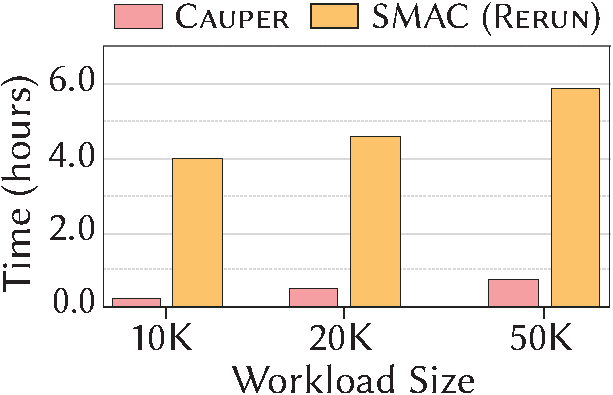
\includegraphics[width=0.45\linewidth]{fig__rq3_e.pdf}
%         \label{fig:rq3_2_b}
%     }
%     \caption{\small \tool vs. SMAC for varying workload. \tool is less sensitive to workload changes.}% (indicated by $\blacklozenge$).}
%     \label{tab:rq3_2}
% \end{figure}

% \motivation
% In this paper, we study fault diagnostic, \ie, situations where a misconfiguration has resulted in non-performance faults, and tools such as  \tool are used to diagnose the root causes and recommend fixes for the misconfiguration. An alternate approach is to use configuration optimization, where the goal is to automatically tune a system by discovering a ``near-optimum'' configuration. 





% \subsubsection*{\textbf{Motivation.}} Search based methods use techniques such as Bayesian optimization~\cite{snoek2012practical, shahriari2015taking} to explore the relationships between configuration options and corresponding non-functional properties. 
% % Unlike machine learning models, optimization methods build and iteratively improve a surrogate model. The balance between exploration (to increase sample diversity) and exploitation (to measure configuration in interesting regions) in the hope of finding a ``near-optimal'' configuration. 
% Albeit recent approaches seem promising~\cite{hsu2018arrow, dalibard2017boat, miyazaki2018bayesian}, these methods are not viable for diagnostics since our objective is not to find an optimal configuration, rather it is to fix an already encountered fault. In this RQ, we explore the challenges of using optimization for fault diagnostics in terms of their efficacy (RQ2-A), their analysis time (RQ2-B), and their sensitivity to external changes (RQ2-C), 
% by comparing \tool with two popular optimization approaches: (a) SMAC and (b) PESMO (see~\tion{baselines}). 


% The assume the software stack to be 
% The prior captures beliefs about the behavior of the function
% decide where to sample to update the 
% model

% to efficiently search the 
% configuration space 

% In this section, we compare \tool with configuration optimization techniques, where the goal is to automatically tune a system by discovering a ``near-optimum'' configuration. Diagnostics (with tools like \tool) and optimization are tangential to one another. Diagnostics fix an already encountered fault, whereas optimization searches the configuration space for a near-optimal configuration. In this section, we contrast the two approaches to understand the challenges of using optimization for fault diagnostics. 

% \approach 
% % \bisq
% % \item \textsc{SMAC}~\cite{hutter2011sequential}: A sequential model based optimization technique to auto-tune software systems; 
% % \item \textsc{PESMO}~\cite{hernandez2016predictive}: A multi-objective bayesian optimization to find an near-optimum configuration.
% % \ei
% % We compare \tool with the following two optimization techniques:
% % 
% % 
% % \besq
% % \item How effective is optimization?
% % % \item How effective is multi-objective optimization?
% % \item What is the analysis time of optimization and \tool?
% % \item How sensitive is optimization to workload changes?
% % % \item Can optimization be used to augment diagnostics?
% % \ee
% % 
% We use latency faults from our benchmark from Image recognition deployed on Jetson \txtwo. There were a total of 21 such faults. Our findings generalize over other combinations of software and hardware.
% 
% 




% \begin{figure}[t]
%     \setlength{\belowcaptionskip}{-1.5em}
%     % \subfloat[\tool vs. SMAC for resolving \\latency faults.]{
%     %     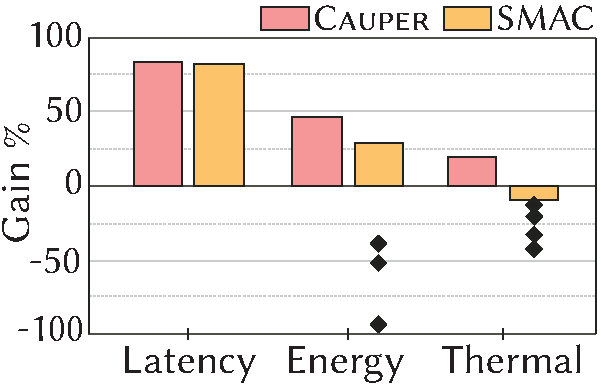
\includegraphics[width=0.3\linewidth]{fig__rq3_a.pdf}
%     %     \label{fig:rq3_1_a}
%     % }\quad
%     \subfloat[\textsc{Xception}]{
%         \includegraphics[width=0.48\linewidth]{figures-vg/Image_sample_energy_gain.pdf}
%         \label{fig:rq2_energy_xception}
%     }
%     % \subfloat[Multi Objective]{
%     %     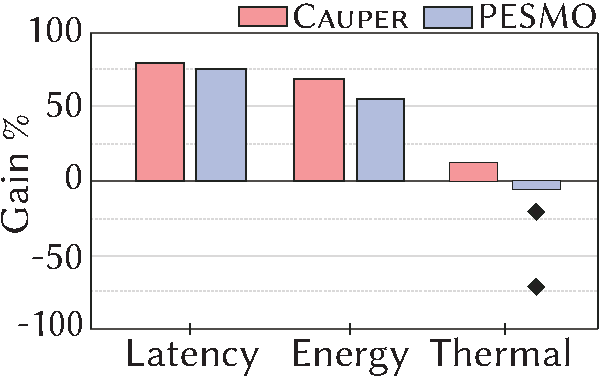
\includegraphics[width=0.275\linewidth]{fig__rq3_b.pdf}
%     %     \label{fig:rq3_1_b}
%     % }
%     \subfloat[\textsc{BERT}]{
%         \includegraphics[width=0.48\linewidth]{figures-vg/NLP_sample_energy_gain.pdf}
%         \label{fig:rq2_energy_bert}
%     }
    
%     \subfloat[\textsc{Deepspeech}]{
%         \includegraphics[width=0.48\linewidth]{figures-vg/Speech_sample_energy_gain.pdf}
%         \label{fig:rq2_energy_deepspeech}
%         }
%         \subfloat[\textsc{x264}]{
%             \includegraphics[width=0.48\linewidth]{figures-vg/x264_sample_energy_gain.pdf}
%             \label{fig:rq2_energy_x264}
%     }
%     \caption{\small{Sample efficiency of \tool in debugging non-functional energy faults}}% (indicated by $\blacklozenge$).}}
%     \label{tab:rq2_2}
% \end{figure}

% \begin{figure*}[t!]
%     % \setlength{\belowcaptionskip}{-3em}
%     \centering
%     \includegraphics*[width=\linewidth]{figures-vg/latency_eff.pdf}
%     \vspace{-3em}
%     \caption{\small{Sample efficiency of \tool in debugging non-functional latency faults}}
    
%     \label{fig:rq2_1}
%     % \rayb{I have questions about this figure. Let's talk in the morning}
% \end{figure*}

% \begin{figure*}[t!]
%     % \setlength{\belowcaptionskip}{-3em}
%     \centering
%     \includegraphics*[width=\linewidth]{figures-vg/energy_eff.pdf}
%     \vspace{-3em}
%     \caption{\small{Sample efficiency of \tool in debugging non-functional energy faults}}
    
%     \label{fig:rq2_2}
%     % \rayb{I have questions about this figure. Let's talk in the morning}
% \end{figure*}
%\subsection{RQ2: How sample efficient is \tool for different performance tasks?}

% \section{Sample Efficiency (RQ2)} 
% % In this RQ, we investigate the sampling efficiency of \tool for different performance tasks. 
% %To answer this RQ, it is sufficient to study \tool for debugging non-functional fault tasks in the SE setting as this generalizes over performance tasks.
% Here, we only study \tool for debugging \textsc{nf-fault} task as this generalizes over performance tasks.

% \noindent \textbf{Setting}.
% We use the same setting for debugging single-objective latency and energy faults for \tool. For other baseline methods, we evaluate the performance gains with varying sample sizes. 

% \noindent \textbf{Results.}
% This issue is compounded when performing multi-objective optimization.% adding to the overall inference time considerably. 

% \tool required a higher number of samples to resolve the latency and energy faults in \textsc{x264} and \textsc{Deepspeech}, respectively when compared to other systems. 
% \bugdoc always achieves a higher gain with the initial 25 number of samples. However, with a higher number of samples, \bugdoc has a slower increase than methods like \textsc{DD} or \textsc{Encore}. 


%~\rayb{Can you explain why causal analysis requires less sample in 1/2 lines?}
\begin{figure}[tp!]
    \setlength{\belowcaptionskip}{-1.5em}
    \centering
    \includegraphics*[width=\linewidth]{figures-vg/barplot_multi_debug_orig.pdf}
    % \includegraphics*[width=0.24\linewidth]{figures-vg/barplot_multi_debug_orig_time.pdf}
    \caption{\small{{\ourapproach has higher accuracy, precision, recall, and gain in debugging non-functional energy faults when hardware changes (\xavier to \txtwo)}}.}% (indicated by $\blacklozenge$).}}
    \label{fig:rq1_debugging_multi}
\end{figure}
% \begin{tcolorbox}
% \textbf{Summary.} \tool is sampling efficient for different performance tasks. 
% \end{tcolorbox}

\begin{figure}[tp!]
    % \setlength{\belowcaptionskip}{-3em}
    \centering
    \includegraphics*[width=\linewidth]{figures-vg/barplot_multi_opt.pdf}
    \caption{\small {\ourapproach finds configurations with higher gain when workloads are changed for performance (latency) optimization task in \txtwo.}}
    
    \label{fig:rq1_opt_me}
    % \rayb{I have questions about this figure. Let's talk in the morning}
\end{figure}

\section{Transferability} 
\label{sec:transfer}

% In this RQ, we investigate the transferability of \tool for different performance tasks. 
%To answer this RQ, it is sufficient to study \tool for debugging non-functional fault task in the SE setting as this generalizes over performance tasks.

% \noindent \textbf{Task1. Debugging \& Repair}.

\noindent \textbf{Setting.} We reuse the causal performance model constructed from a source environment, e.g., \txone, to resolve a non-functional fault in a target environment, e.g., \xavier. We evaluated \ourapproach for debugging energy faults for \textsc{Xception} and used \xavier as the source and \txtwo as the target, since they have different microarchitectures, expecting to see large differences in their performance behaviors. We only compared with \bugdoc as it discovered fixes with higher energy gain in \xavier than other correlation-based baseline methods (see ~\Cref{tab:single_1}). We compared \ourapproach and \bugdoc in the following scenarios: (i) \bugdoc (\textsc{Reuse}) and \ourapproach (\textsc{Reuse}): reusing the recommended configurations from Source to Target, (ii) \bugdoc \textsc{+ 25} and \ourapproach \textsc{+ 25}: reusing the performance models (i.e., causal model and decision tree) learned in Source and fine-tuning the models with 25 new samples in Target, and (iii) \bugdoc (\textsc{Rerun}) and \ourapproach (\textsc{Rerun}): we rerun \ourapproach and \bugdoc from scratch to resolve energy faults in Target. %In both settings, we use relevance score, $\Delta_{gain}$ and wallclock time to determine the effectiveness of \tool. Fig. \ref{fig:acc_shd_iter} indicates how the SCM structure converges to the approximate true causal structure. Here, the structural hamming distance (SHD) value decreases with incremental learning. Fig. \ref{fig:incremental_update} shows how the new recommended configuration from the incremental learning stage resolves the fault and finds the root cause. 
For optimization tasks, we use three larger additional \textsc{Xception} workloads: 10000 (10k), 20000 (20k), and 50000 (50k) test images (previous experiments used 5000 (5k) test images). We evaluated three variants of SMAC and \ourapproach: 
(i)~SMAC (\textsc{Reuse}) and \ourapproach (\textsc{Reuse}), where we \textit{reuse} the near-optimum found with 5k test images on the larger workloads; 
(ii)~SMAC + 10\% and \ourapproach + 10\%, where we rerun with 10\% budget in target and update the optimization and causal performance model with 10\% additional budget; and
(iii)~SMAC + 20\% and \ourapproach + 20\%, where we rerun with 20\% budget in target and update the models with 20\% additional budget.


\noindent \textbf{Results.} 
\fig{rq1_debugging_multi} indicates the results in resolving energy faults in \txtwo. We observe that \ourapproach + 25 obtains 8\% more accuracy, 7\% more precision, 5\% more recall and 8\% more gain than \bugdoc \textsc{(Rerun)}. Here, \bugdoc takes significantly longer time than \ourapproach, \ie, \bugdoc (\textsc{Rerun}) exhausts the entire 4-hour budget whereas \ourapproach takes at most 20 minutes to fix the energy faults. Moreover, we have to rerun \bugdoc every time the hardware changes, and this limits its practical usability. In contrast, \ourapproach incrementally updates the internal causal model with new samples from the newer hardware to learn new relationships. We also observe that with little updates, \ourapproach + 25 ($\sim$20 minutes) achieves a similar performance of \ourapproach \textsc{(Rerun)} ($\sim$36 minutes). Since the causal mechanisms are sparse, the causal performance model from \xavier in \ourapproach quickly reaches a fixed structure in \txtwo using incremental learning by judiciously evaluating the most promising fixes until the fault is resolved.

Our experimental results demonstrate that \ourapproach performs better than the two variants of three SMAC (c.f. \fig{rq1_opt_me}). SMAC (\textsc{Reuse}) performs the worst when the workload changes. With 10K images, reusing the near-optimal configuration from 5K images results in a latency gain of 10\%, compared to 12\% with \ourapproach in comparison with the default configuration. We observe that \ourapproach + 20\% achieves 44\%, 42\%, and 47\% higher gain than SMAC + 20\% for workload sizes of 10k, 20k, and 50k images, respectively. 


% \noindent \textbf{Results}.
% In the earlier RQ, we observed \tool had higher gain and lower hypervolume errors for single and multi-objective optimization, respectively for both settings that can be explained by the results presented in Table. \tool sampled a higher number of better configurations than other approaches and achieved higher gain. Optimization approaches are non-causal and sampled a lower number of configurations as they sampled some costly configurations that had little or no gain. 
% \noindent \textbf{Single-environmental setting results.}
% The analysis time of all approaches are reported in~\fig{rq3_1_c}. Optimization methods run until they converge, however it is a common practice to assign a maximum budget (we use 4 hours) to limit inference time and cost. \tool was found to have comparatively lesser inference time compared to the other methods. While SMAC takes slightly more than 3 hours to find a near-optimum in \txtwo (image recognition), \tool resolved the faults in 20 minutes on average ($9\times$ faster). Likewise, PESMO takes close 4 hours compared to 45 minutes with \tool ($5\times$ faster). 

% \noindent \textbf{Multi-environmental setting results.}
% In \fig{rq3_1_e} we report the inference times for SMAC (\textsc{Rerun}) and \tool. In keeping with the previous results, SMAC (\textsc{Rerun}) takes significantly longer than \tool, \ie, SMAC (\textsc{Rerun}) exceeds the 4 hour budget in all workloads whereas \tool takes at most 30 minutes for the largest workload to diagnose and fix the latency faults. We have to rerun SMAC every time the workload changes, and this limits its practical usability. In contrast, \tool incrementally updates the internal causal model with new samples from the larger workload to learn new relationships from the larger workload. Therefore, it is less sensitive and much faster. 
% Since \tool uses causal models to infer candidate fixes using only the available observational data, it tends to be much faster than SMAC and PESMO. During incremental learning, \tool judiciously evaluates the most promising fixes until the fault is resolved. This limits the number of times the system is reconfigured and profiled. In contrast, optimization techniques sample several sub-optimal configurations in their search process and they are all evaluated. 


% \begin{tcolorbox}
% \textbf{Summary.} \tool is transferable across environments for different performance tasks. 
% \end{tcolorbox}

%\subsection{RQ3: How scalable is \tool for growing configuration spaces for different performance tasks?}

\begin{table}[tp!]
    % \setlength{\belowfloatskip}{-1.5em}
%\caption{Scalability of \tool for \textsc{sqlite} and \textsc{Deepstream} on \xavier.}
\caption{Scalability for \textsc{SQLite} and \textsc{DeepStream} on \xavier.}
\label{tab:scalability}
% \subfloat[Larger number of configuration options.]{
\resizebox{0.98\linewidth}{!}{
\begin{tabular}{V{2}rrrrrrrV{2}rrrV{2}}
\clineB{8-10}{2}
\multicolumn{1}{l}{}              & \multicolumn{1}{l}{}   & \multicolumn{1}{l}{}           &
\multicolumn{1}{l}{}           &
\multicolumn{1}{l}{}           &
\multicolumn{1}{l}{}         & \multicolumn{1}{cV{2}}{}              & \multicolumn{3}{cV{2}}{Time/Fault (in sec.)}                                                    \bigstrut\\ \clineB{1-7}{2}
\multicolumn{1}{V{2}r}{\rotatebox{90}{System}} &{\rotatebox{90}{Configs}}&
{\rotatebox{90}{Events}} &\multicolumn{1}{r}{\rotatebox{90}{Paths}} & \multicolumn{1}{r}{\rotatebox{90}{Queries}} &
\multicolumn{1}{r}{\rotatebox{90}{Degree}} &
\multicolumn{1}{rV{2}}{\rotatebox{90}{Gain (\%)}} & \multicolumn{1}{r}{\rotatebox{90}{Discovery}} & \multicolumn{1}{r}{\rotatebox{90}{Query Eval}} & \multicolumn{1}{rV{2}}{\rotatebox{90}{\bfseries Total}} \bigstrut\\ \hlineB{2}

\multicolumn{1}{c}{}& \multicolumn{1}{c}{}&\multicolumn{1}{c}{}& \multicolumn{1}{c}{}& \multicolumn{1}{c}{}& \multicolumn{1}{c}{}& \multicolumn{1}{c}{}& \multicolumn{1}{c}{}\bigstrut\\[-1.5em] \hlineB{2}

\multicolumn{1}{V{2}r}{\textsc{SQLite}}   & \multicolumn{1}{r}{34}  & \multicolumn{1}{r}{19}                    & \multicolumn{1}{r}{32}        & \multicolumn{1}{r}{191} &   \multicolumn{1}{r}{3.6} & 93                              & 9                            & 14                            & \cellcolor{blue!10}\textbf{291}                     \bigstrut\\ 
\multicolumn{1}{V{2}r}{}    & \multicolumn{1}{r}{242}  & \multicolumn{1}{r}{19}                   & \multicolumn{1}{r}{111}       & \multicolumn{1}{r}{2234}   & \multicolumn{1}{r}{1.9}& 94                               & 57                           & 129                           & \cellcolor{blue!10}\textbf{1345}                    \bigstrut\\
% \multicolumn{1}{V{2}r}{136}                    & \multicolumn{1}{r}{441}       & \multicolumn{1}{r}{8341}    & 93                             & 111                         & 381                             & \cellcolor{blue!10}\textbf{2817}           \bigstrut\\
% \multicolumn{1}{c}{}& \multicolumn{1}{c}{}& \multicolumn{1}{c}{}& \multicolumn{1}{c}{}& \multicolumn{1}{c}{}& \multicolumn{1}{c}{}& \multicolumn{1}{c}{}\bigstrut\\[-1.5em] \hlineB{2}
\multicolumn{1}{V{2}r}{}&  \multicolumn{1}{r}{242} & \multicolumn{1}{r}{288}                      & \multicolumn{1}{r}{441}       & \multicolumn{1}{r}{22372} & \multicolumn{1}{r}{1.6}    & 92                             & 111                         & 854                             & \cellcolor{blue!10}\textbf{5312}           \bigstrut\\ \hlineB{2}
\multicolumn{1}{V{2}r}{\small \textsc{Deepstream}}   & \multicolumn{1}{r}{53}  & \multicolumn{1}{r}{19}                    & \multicolumn{1}{r}{43}        & \multicolumn{1}{r}{497} &   \multicolumn{1}{r}{3.1} & 86                              & 16                            & 32                            & \cellcolor{blue!10}\textbf{1509}                     \bigstrut\\ 

\multicolumn{1}{V{2}r}{}&  \multicolumn{1}{r}{53} & \multicolumn{1}{r}{288}                      & \multicolumn{1}{r}{219}       & \multicolumn{1}{r}{5008} & \multicolumn{1}{r}{2.3}    & 85                             & 97                         & 168                             & \cellcolor{blue!10}\textbf{3113}           \bigstrut\\ \hlineB{2}


\end{tabular}}\vspace{-1em}

\end{table}

\section{Scalability}
\label{sec:scalability}

% Scalability of \tool depends on the scalability of each phase. Therefore, we design scenarios to test the scalability of each phase to determine the overall scalability. Since the initial number of samples and the underlying phases for each task is the same, it is sufficient to examine the scalability of \tool for the debugging non-functional fault task. 

 
% \textsc{sqlite} was chosen because it offers a large number of configurable options, much more than  DNN-based applications, and video encoders. Further, each of these options can take on a large number of permitted values making \textsc{Deepstream} a useful candidate to study the scalability of \tool. \textsc{Deepstream} was chosen as it has a higher number of components than others and it is interesting to determine how \tool behaves when the number of options and events are increasing.
% As a result, SQLite exposes new system design opportunities to enable efficient inference and many complex interactions between software options. 
% We evaluate \tool under two scalability scenarios: (1) larger configuration space (RQ3-A), and (2) more granular values for each configuration option (RQ3-B). 

% \noindent\textbf{RQ3-A.~How does \tool scale with a larger number of configuration options?} 
\noindent{\textbf{Setting.}}~ We evaluated \ourapproach for scalability with \textsc{SQLite} (large configuration space) and \textsc{Deepstream} (large composed system). %The causal graphs of DNN based systems used 47 variables with 34 hardware, kernel/OS, and software configuration options in addition to 19 system events.
In \textsc{SQLite}, we evaluated three scenarios: (a)~selecting the most relevant software, hardware options, and events (34 configuration options and 19 system events), (b) selecting all modifiable software and hardware options and system events (242 configuration options and 19 events), and (c) selecting not only all modifiable software and hardware options and system events but also intermediate {\tt tracepoint events} (242 configuration options and 288 events). In \textsc{Deepstream}, there are two scenarios: (a) 53 configuration options and 19 system events, and (b) 53 configuration options and 288 events when we select all modifiable software and hardware options, and system/tracepoint events. %For each scenario, we track the time required to discover the causal structure, evaluate the counterfactual queries, and total time to resolve throughput faults. 


\noindent{\textbf{Results.}} In large systems, there are significantly more causal paths and therefore, causal learning and estimations of queries take more time. %However, with as much as 242 configuration options and 19 events (\tab{scalability}, row 2), causal graph discovery takes roughly one minute, evaluating all 2234 queries takes roughly two minutes, and the total time to diagnose and fix a fault is roughly 22 minutes for \textsc{sqlite}. This trend is observed even with 242 configuration options, 288 events (\tab{scalability}, row 3), and finer granularity of configuration values---the time required to causal model recovery is a little over 1 minute and the total time to diagnose and fix a fault is less than 2 hours. Similarly in \textsc{Deepstream}, with 53 configuration options and 288 events, causal model discovery is less than two minutes and the time needed to diagnose and fix a fault is less than an hour. 
The results in ~\tab{scalability} indicate that \ourapproach can scale to a much larger configuration space without an exponential increase in runtime for any of the intermediate stages. This can be attributed to the sparsity of the causal graph. For example, the average degree of a node for \textsc{SQLite} in \tab{scalability} is at most 3.6, and it reduces to 1.6 when the number of configurations increases. Similarly, the average degree reduces from 3.1 to 2.3 in \textsc{Deepstream} when systems events are increased. %This makes sense because not all variables (\ie, configuration options and/or system events) affect non-functional properties and a high number of variables in the graph end up as isolated nodes. Therefore, the number of paths and consequently the evaluation time do not grow exponentially as the number of variables increases.

% To understand how \tool scales in such scenarios, we evaluate \tool by increasing the number of values the software, hardware, and kernel configuration options can be set to while resolving the latency faults in the SQLite. From \tab{scalability} we observe that even with 242 configurations, 288 events (\tab{scalability}, row 3), and finer granularity of configuration values, the time required to causal model recovery is less than two minutes and the total time to diagnose and fix a fault is less than 2 hours. We also observe that the graph becomes more sparse (average degree of a node decreases from 1.8 to 1.6 in \tab{scalability}) and the evaluation time does not grow exponentially. 

% Finally, the latency gain associated with repairs from larger configuration space with configurations was similar to the original space of 34 and 53 configurations for \textsc{sqlite} and \textsc{Deepstream}, respectively. This indicates that: (a)~imparting domain expertise to select most important configuration options can speed up the inference time of \tool, and (b)~if the user chooses instead to use more configuration options (perhaps to avoid initial feature engineering), \tool can still diagnose and fix faults %satisfactorily within a reasonable time. 

% To understand how \tool scales in such scenarios, we evaluate \tool by increasing the number of values the software, hardware, and kernel configuration options can be set to while resolving the latency faults in the SQLite. %There are two scenarios in this case: (a) 242 configurations and 88 system events when we select all the modifiable software/hardware configurations and events and (b) 242 configurations and 288 events when we select not only all modifiable software and hardware configurations and system events but also intermediate {\tt tracepoint events}. 
% In the second case, we increase the granularity of kernel configurations by considering all the permitted values by \texttt{Linux} kernel. As system events can only be observed, we increase the granularity of events by observing the tracepoint events along with hardware/software events. 
% Similar to {RQ3-A.}, we track the time required to discover the causal structure, evaluate the counterfactual queries, and total time to resolve latency faults.
% 


% In summary, 

% x